
\documentclass[11pt]{scrartcl}

\usepackage[spanish]{babel}
\usepackage[utf8]{inputenc}

\usepackage[parfill]{parskip}
\usepackage{schemata}
\usepackage{caption}
\usepackage{subcaption}

% \setlength{\parindent}{0pt}
% \setlength{\parskip}{1.1ex plus 0.5ex minus 0.2ex}

\usepackage{graphicx}
\usepackage{longtable}
\usepackage{float}

\usepackage{multirow}
\usepackage{minted}
\usepackage{soul}
\usepackage{amssymb}
\usepackage{hyperref}

\usepackage{amsmath}
\usepackage{amsthm}
\usepackage{mathtools}
\usepackage{tabularx}
\usepackage{wrapfig}
\usepackage{rotating}
% \usepackage{inconsolata}

\usepackage{color}
\usepackage{framed}
\definecolor{prueba}{rgb}{.1,.1,.4}
\hypersetup{colorlinks=true, linkcolor=prueba,citecolor=prueba, filecolor=prueba, menucolor=prueba, urlcolor=prueba}
\usepackage{float}

\usepackage{fancyvrb}
%\renewcommand{\familydefault}{\sfdefault}

\usepackage[top=2.1cm, bottom=2.1cm, left=2.1cm, right=2.1cm]{geometry}

% Spacing de las matrices
\renewcommand*{\arraystretch}{1.5}

\title{\Huge{Apuntes}\\[0.2cm]\LARGE{Reconocimiento de Patrones}}
\author{José Tomás Tocino García}
\date{Junio de 2013}

\newenvironment{ejemplo}%
{\VerbatimEnvironment\begin{Verbatim}[frame=single]}%
{\end{Verbatim}}%

\definecolor{matlabcode_bg}{rgb}{0.95,0.95,0.95}
\newminted{matlab}{bgcolor=matlabcode_bg, baselinestretch=1.05}


\begin{document}

\maketitle

\tableofcontents

\pagebreak

\section{Introducción a la asignatura}

El \textbf{reconocimiento de patrones} trata las técnicas de análisis y
extracción de información de elementos, tanto físicos como lógicos, con objeto
de establecer propiedades, clasificaciones y reglas sobre dichos objetos -- esto
es, identificar \textbf{patrones}, con los que llevar a cabo multitud de
funciones.

\subsection{Convenciones sobre los datos}

Se han seguido ciertas convenciones a la hora de presentar y trabajar con los
datos. Un \textbf{patrón} es un conjunto de valores relacionados que
\textit{definen} a un \textbf{individuo} de una población. Un patrón se
representa con un \textbf{vector columna}, en el cada \textbf{característica}
ocupa una fila. Este vector se conoce como \textbf{vector de características}.

$$
x = \begin{bmatrix}
x_1 \\
x_2 \\
x_3 
\end{bmatrix}
$$


Los \textbf{patrones} se presentarán de forma matricial con la letra $X$,
ocupándose \textbf{una columna por patrón}. 

$$
X = \begin{bmatrix}
x_{11} & \ldots & x_{1n} \\
x_{21} & \ldots & x_{2n} \\
x_{31} & \ldots & x_{3n}
\end{bmatrix}
$$

Por ejemplo, si estamos en una clase con 6 alumnos y a cada uno (cada
\textit{patrón}) le medimos la altura y el peso (las \textit{características}),
la matriz resultante tendría dos filas y 6 columnas:

$$
X = \begin{bmatrix}
1.70 & 1.90 & 1.80 & 1.73 & 2.01 & 1.65 \\
70   & 90   & 80   & 81   & 97   & 54
\end{bmatrix}
$$

Por otro lado, tendremos una serie de \textbf{clases} entre las que dividir
nuestros datos. En el ejemplo, las dos clases podrían ser \textbf{hombre} y
\textbf{mujer}, por ejemplo. La clases también se representan de forma
matricial, con la letra $Y$, que contendrá una fila (la \textit{clase}) y tantas
columnas como patrones. 

Normalmente las clases se \textbf{codifican} de forma numérica, asigando (por
ejemplo) el número 1 a la clase \textit{hombre} y el 2 a la clase
\textit{mujer}:

$$
Y = \begin{bmatrix}
2 & 2 & 1 & 2 & 1 & 2
\end{bmatrix}
$$



\section{Clasificación}

Una de las principales funciones del reconocimiento de patrones es la
\textbf{clasificación} de patrones utilizando la información proporcionada por
otros patrones previamente clasificados de forma correcta. Se suele recibir un
conjunto de patrones de entrenamiento, junto a sus clases, y un conjunto de
patrones de test, para los que calcular la clase. Estudiaremos diversos métodos
para la clasificación.

\subsection{Diagrama de métodos de clasificación}

Se listan los métodos de clasificación estudiados, según el tipo de cada uno.

\bigskip

\schema
{%
  \schemabox{Métodos de\\ clasificación}
}
{%
  \schema
  {%
    \schemabox{Métodos paramétricos \\ 
      \scriptsize Para cada clase obtienen \\
      \scriptsize una serie de parámetros \\ 
      \scriptsize que la caracterizan}
  }
  {%
    \schema
    {
      \schemabox{Dist. mínima}
    }
    {
      \schema
      {
        \schemabox{1 centro/clase}
      }
      {
        \schemabox{Distancia euclídea}
        \schemabox{Distancia manhattan}
        \schemabox{Distancia mahalanobis}
      }

      \schema
      {
        \schemabox{$N$ centros/clase}
      }
      {
        \schemabox{K-medias}
      }
    }
  }

  \schema
  {%
    \schemabox{Métodos no paramétricos \\
      \scriptsize Usan directamente los datos \\
      \scriptsize de entrada para clasificar \\
      \scriptsize los patrones
    }
  }
  {
    \schemabox{1-NN: 1-vecino más cercano}
    \schemabox{K-NN: K-vecinos más cercanos}
  }
}

\subsection{Método de la distancia mínima}

El método de la \textbf{distancia mínima} clasifica los patrones según su
\textbf{distancia} hacia unos puntos, conocidos como \textbf{prototipos}, que
representarán las clases. Hay múltiples formas de \textbf{decidir los
  prototipos}, así como diferentes maneras de \textbf{calcular las distancias}
hacia esos centros.

En general, el \textbf{algoritmo} de la distancia mínima sigue los siguientes
pasos:

\begin{enumerate}
\item Calcular los centros para cada clase.
\item Calcular la distancia entre cada patrón y cada clase.
\item Asignar a cada patrón la clase cuyo centro tiene más cerca.
\end{enumerate}

\subsection{Selección del prototipo}

Seleccionar el \textbf{prototipo} para cada clase es el primer paso del
procedimiento. Al igual que los patrones, un prototipo se representa como un
vector de características.

Es habitual calcular el prototipo de una clase como la \textbf{media de los
  patrones} pertenecientes a esa clase, fila a fila. Esto es, el valor de la
característica $c$ del prototipo será la media de los valores para $c$ de los
patrones de esa clase.

En Matlab, el cálculo del prototipo de una clase $c$ se hace de la siguiente manera:

\begin{matlabcode}
% Decidimos la clase para la que generar el prototipo
clase = 1; 

% Aislamos los patrones de esa clase
x_aux = x(:, y == clase);  

% Hacemos la media de las filas de esos patrones
prototipo = mean(x_aux, 2);

% O usando la biblioteca 'pattern'
prototipo = meanpat(x_aux);
\end{matlabcode}

\subsection{Distancia euclídea}

La forma más básica del algoritmo utiliza la \textbf{distancia euclídea} para
calcular la distancia entre los patrones y los prototipos de las clases. La
distancia euclídea es la distancia más habitual, ya que se ajusta a la idea
intuitiva de \textit{distancia}.

La distancia euclídea entre un patrón $x$ y un prototipo $p$ se calcula como:

$$
d(x,p) = \sqrt{(x_1 - p_1)^2 + (x_2 - p_2)^2 + \dots + (x_n - p_n)^2}
$$

En Matlab, la distancia euclídea de un conjunto de patrones a un prototipo se
puede calcular usando la función \texttt{d\_euclid} de la biblioteca
\texttt{pattern}:

\begin{matlabcode}
% Suponemos que tenemos tres clases
for i = 1:3
  distancias(i,:) = d_euclid(x, prototipos(:, i));
end
\end{matlabcode}

O también manualmente, utilizando la función \texttt{norm}:

\begin{matlabcode}
for i = 1:3
  for j = 1:size(x,2)
    distancias(i,j) = norm(x(:, j) - prototipo(:, i))
  end
end
\end{matlabcode}

Conocidas las distancias de cada punto a cada prototipo, solo queda seleccionar
el prototipo más cercano a cada punto y así decidir su clase. En Matlab:

\begin{matlabcode}
% Por defecto calcula los minimos por columnas
[~, pos] = min(distancias);  
\end{matlabcode}

\subsection{Distancia de Manhattan}

La \textbf{distancia de Manhattan} recibe ese nombre porque es la habitualmente
usada en ciudades con una distribución en rejilla como Manhattan. El cálculo de
esta distancia es sencillo: utiliza la suma de las diferencias, en valor
absoluto, de las componentes de los vectores a comparar. Así, la distancia entre
un patrón $x$ y un prototipo $p$ se define como:

$$
d(x,p) = |x_1 - p_1| + |x_2 - p_2| + \dots + |x_n - p_n| = \sum^n_{i=1} |x_n - p_n|
$$

El cálculo en Matlab se puede hacer de la siguiente manera:

\begin{matlabcode}
for i = 1:numClases
  % Convertimos el prototipo en una matriz con columnas iguales
  aux = repmat(prototipo(:, i), 1, length(x));
  
  distancias(i,:) = sum(abs(x - aux))
end
\end{matlabcode}

\subsection{Distancia de Mahalanobis}

Existen situaciones en las que las distancias anteriores no funcionan bien,
porque no tienen en cuenta más que la diferencia entre los valores de los
patrones y los prototipos, pero no su rango, varianza ni ninguna otra cualidad.

Por ejemplo, supongamos un sistema en el que los patrones tienen dos
características, $c_1$ y $c_2$. $c_1$ suele variar entre 0 y 100 y $c_2$ entre
10 y 15. La distancia euclídea y la de Manhattan no tienen en cuenta el rango de
las características, por lo que si un patrón tiene $c_2 = 10$ y el prototipo
tiene $c_2 = 15$, su distancia no será grande, aun a pesar de que la segunda
característica es \textit{totalmente} diferente.

Para solventar este problema resulta necesario incluir en el cálculo de la
distancia algún otro parámetro que caracterice cada característica.

\subsubsection{Matriz de covarianza}

En un entorno unidimensional, la \textbf{desviación típica} (que suele
representarse como $\sigma$) mide la \textit{dispersión} de los datos respecto
al valor medio. Por ejemplo, las tres muestras $(0, 0, 14, 14)$, $(0, 6, 8, 14)$
y $(6, 6, 8, 8)$ cada una tiene una media de 7. Sus desviaciones estándar son
8.08, 5.77 y 1.15 respectivamente. La tercera muestra tiene una desviación mucho
menor que las otras dos porque sus valores están más cerca de la media, que es
7.

La \textbf{varianza} es el cuadrado de la desviación típica, se denota como
$\sigma^2$ y es una medida alternativa de la dispersión, utilizada para
facilitar ciertos cálculos.

En un entorno multidimensional, la \textbf{covarianza} mide la relación entre
dos variables a la hora de crecer o decrecer. La \textbf{matriz de covarianza},
que se denota con $C$, es una matriz \textbf{simétrica} que guarda información
sobre cómo se distribuyen las variables de un conjunto, tanto a nivel individual
como a pares. En su \textbf{diagonal} se encuentra la \textbf{varianza} de cada
una de las variables. El resto de celdas describe la \textbf{relación} entre
cada par de variables, definidas del siguiente modo:

\begin{itemize}
\item Si $C(i,j)>0$, ambas características tienden a crecer o decrecer juntas.
\item Si $C(i,j)<0$, cuando una característica crece, la otra decrece.
\item Si $C(i,j)=0$, las características son independientes entre sí.
\end{itemize}

En definitiva:

$$
C = \begin{bmatrix}
\sigma^2_x  & \sigma_{xy} \\
\sigma_{xy} & \sigma^2_y 
\end{bmatrix}
$$

La matriz de covarianza puede calcularse en Matlab mediante el siguiente comando
de la biblioteca \texttt{pattern}:

\begin{matlabcode}
% Matriz de covarianza
C = covpat(x);  
\end{matlabcode}

Que internamente usa la función nativa \texttt{cov}:

\begin{matlabcode}
% cov recibe los patrones por filas, con las caracteristicas por columnas
C = cov(x');
\end{matlabcode}

Ejemplos de matrices de covarianza y la representación de los datos:

\begin{figure}[h!]
 \centering
 \begin{subfigure}{0.49\textwidth}
$$
C = \begin{bmatrix}
1    & 0 \\
0    & 1   
\end{bmatrix}
$$ 
\end{subfigure}
 \begin{subfigure}{0.39\textwidth}
    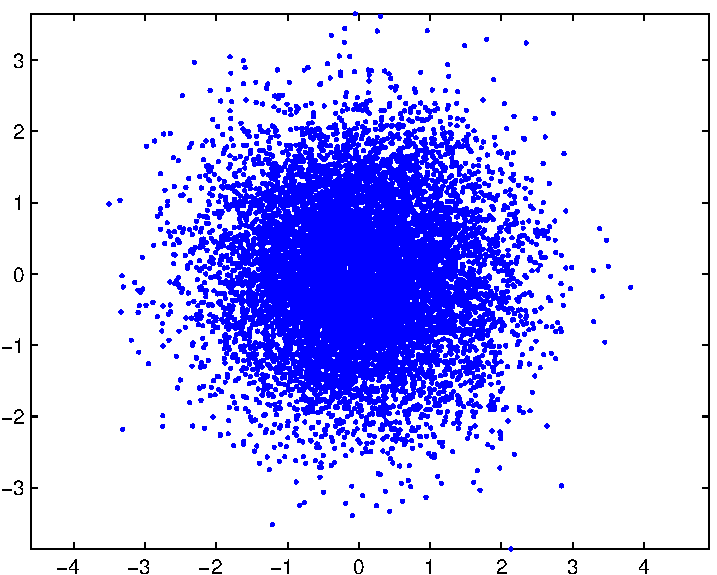
\includegraphics[width=\textwidth]{img/matriz_covarianza_0}
 \end{subfigure}
 \caption{covarianza nula entre variables}
\end{figure}

\begin{figure}[h!]
 \centering
 \begin{subfigure}{0.49\textwidth}
$$
C = \begin{bmatrix}
1    & 0.50 \\
0.50 & 1   
\end{bmatrix}
$$ 
\end{subfigure}
 \begin{subfigure}{0.39\textwidth}
    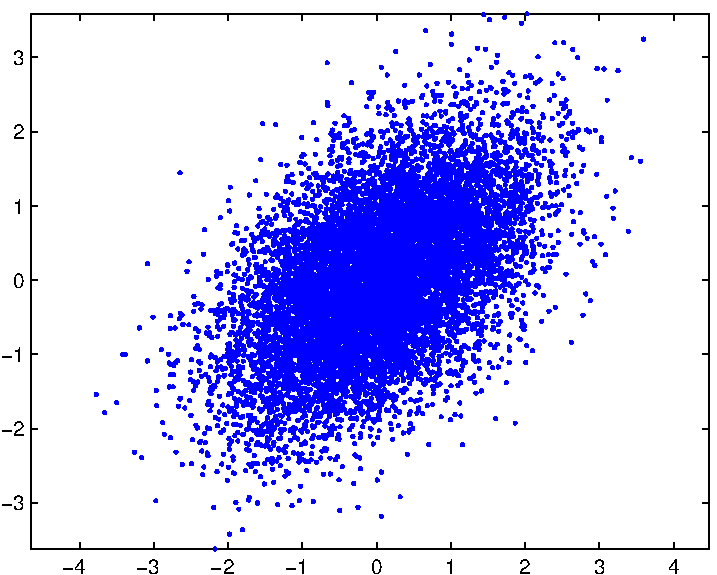
\includegraphics[width=\textwidth]{img/matriz_covarianza_creciente}
 \end{subfigure}
 \caption{covarianza $> 0$, ambas variables crecen a la vez}
\end{figure}

\begin{figure}[h!]
 \centering
 \begin{subfigure}{0.49\textwidth}
$$
C = \begin{bmatrix}
1    & -0.50 \\
-0.50 & 1   
\end{bmatrix}
$$ 
\end{subfigure}
 \begin{subfigure}{0.39\textwidth}
    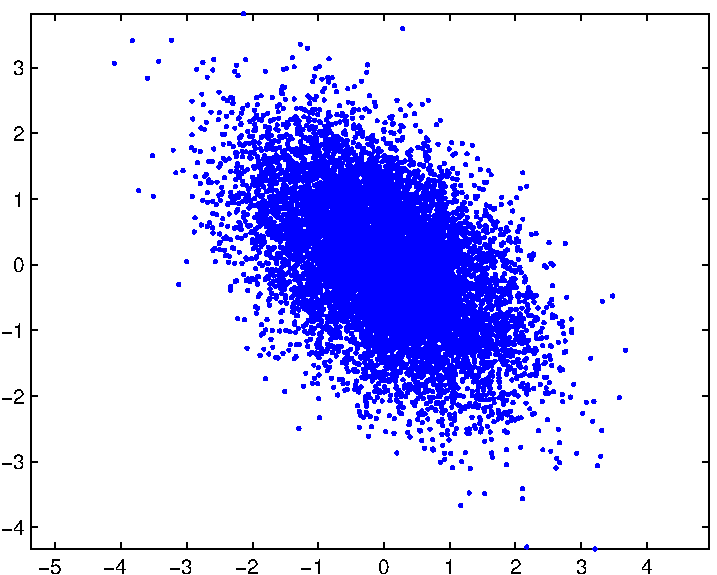
\includegraphics[width=\textwidth]{img/matriz_covarianza_decreciente}
 \end{subfigure}
 \caption{covarianza $< 0$, cuando una var. crece la otra decrece}
\end{figure}

\subsubsection{Aplicación en el cálculo de la distancia}

Una vez conocemos en qué consiste la matriz de covarianza, estudiaremos cómo se
aplica al cálculo de la distancia. En la \textbf{distancia de Mahalanobis}, se
calculará una matriz de covarianza $C_i$ para cada clase. Hecho esto, el cálculo
de la distancia de un patrón $x$ a una clase con prototipo (media) $m_i$ y
matriz de covarianza $C_i$ se define como:

$$
d(x,m,C) = (x-m)' \cdot C^{-1} \cdot (x-m)
$$

Lo que arroja un número, por el producto de matrices. En Matlab, el cálculo de
la distancia de Mahalanobis de un conjunto de patrones $x$ a una clase con media
$m$ y matriz de covarianza $C$ se puede hacer mediante la función
\texttt{d\_mahal} de la biblioteca \texttt{pattern}:

\begin{matlabcode}
for i=1:numClases
  d(i,:) = d_mahal(x, m{i}, C{i});
end  
\end{matlabcode}

Manualmente, podemos hacerlo de la siguiente manera:

\begin{matlabcode}
for i=1:numClases
    for j=1:length(x)
       d(i,j) = ((x(:,j) - m{i})' * inv(C{i}) * (x(:, j) - m{i})); 
    end
end  
\end{matlabcode}

\subsection{K-Medias}

Existen circunstancias en las que la distribución de los puntos de cada clase es
tal que el uso de un solo prototipo por clase \textbf{no es suficiente}, ya que
puede darse que ese prototipo esté demasiado lejos de ciertos puntos, dando
resultados falsos. En esas ocasiones es posible calcular \textbf{varios
  prototipos por clase}.

Las \textbf{k-medias} es un método de agrupamiento que busca dividir una clase
en $k$ grupos, perteneciendo cada patrón al grupo con la media más cercana. El
algoritmo es sencillo:

\begin{enumerate}
\item Elegimos $k$ centros iniciales de entre los patrones.
\item Clasificamos el resto de patrones según la cercanía a los centros.
\item Respecto a la clasificación anterior, calculamos los nuevos centros
  (medias) de cada clase.
\item Volvemos al punto 2.
\item La condición de parada podrá ser un número de iteraciones particular, o la
  convergencia.
\end{enumerate}

\begin{figure}[hc!]
  \centering
  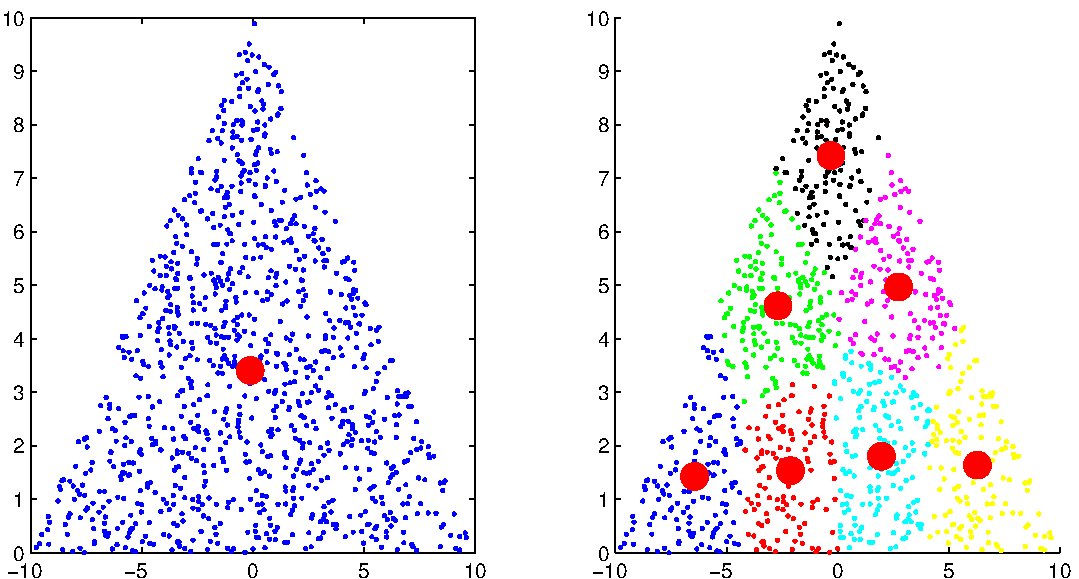
\includegraphics[width=\textwidth]{img/kmedias}
  \caption{Ejemplo con un prototipo, y con k-medias y $k=7$}
\end{figure}

\subsubsection{Implementación}

Una posible implementación del algoritmo de las k-medias en Matlab podría ser la
que sigue:

\begin{matlabcode}
function [ m ] = kmedias( X, numCentros )
% Algoritmo de las K-Medias para X patrones con k prototipos

% Elegimos los k centros iniciales
centros = x(:, randi(length(x), 1, k));

for i=1:50    
    % Vector de distancias
    d = zeros(k, size(x, 2));

    % Calculo las distancias de cada centro a todos los patrones
    for j = 1:k
        d(j,:) = d_euclid(x, centros(:, j));
    end
    
    % Saco el centro mas cercano a cada patron
    [~, yaux] = min(d);
    
    % Genero los nuevos centros
    nuevos_centros = zeros(size(centros));
    for j=1:k       
        nuevos_centros(:, j) = meanpat(x(:, yaux == j));
    end
    
    % Si hay convergencia, terminamos
    if isequal(centros, nuevos_centros)
        centros = nuevos_centros;
        break
    end
    
    centros = nuevos_centros;
end
end
\end{matlabcode}

Y una posible aplicación de esta función podría ser la siguiente, suponiendo
dos poblaciones $xt1$ y $xt2$:

\begin{matlabcode}
K = 5;

% Calculamos los centros
centros_x = [ kmedias(xt1, k) kmedias(xt2, k) ];
centros_y = [ ones(1, k) 2 * ones(1, k) ];

% Calculamos las distancias a los centros
for i=1:k*2
   d(i, :) = d_euclid(xtst, centros_x(:, i)); 
end

% Obtenemos las distancias minimas
[~, pos] = min(d);

fprintf('Errores: %d\n', sum(ytst ~= centros_y(pos)));  
\end{matlabcode}

\subsection{1-NN y k-NN - Vecinos más cercanos}

Hay veces en las que los patrones de las clases están muy solapados entre sí,
por lo que el uso de prototipos para la clasificación no da buenos
resultados. En esos casos es posible utilizar los propios patrones de
entrenamiento como \textit{representantes} de las clases. De ahí, nacen los
métodos basados en los \textbf{vecinos más cercanos} (\textit{NN - Nearest
  neighbors}).

Son métodos \textbf{no paramétricos}, ya que no se basan en un parámetro de la
clase (como pueden ser sus centroides), sino en los propios datos de
entrenamiento.

El \textbf{algoritmo} es muy sencillo. En definitiva, lo que se hace es comparar
el patrón de entrada con todos los patrones de entrenamiento, teniendo en cuenta
la clase del vecino más cercano (o de los \textit{$k$ vecinos} más cercanos)
para decidir la clase del patrón de entrada. Los pasos a seguir son:

\begin{itemize}
\item Se reciben los patrones de entrada.
\item Se calcula la distancia entre el patrón de entrada y todos los patrones de
  entrenamiento.
\item Dependiendo del número de vecinos elegido,
  \begin{itemize}
  \item Si se está usando 1-NN, la clase del patrón de entrada será la misma que
    la del vecino más cercano.
  \item Si se está usando k-NN, la clase del patrón de entrada será la más
    frecuente entre los $k$ vecinos más cercanos.
  \end{itemize}
\end{itemize}

\subsubsection{Implementación}

Una posible implementación puede ser la que sigue:

\begin{matlabcode}
function [ y_test ] = k_vecinos( x_train, y_train, x_test, k)

% Inicializo
y_test = zeros(1,size(x_test,2));

for i = 1:size(x_test, 2)
    % Patttern de test actual
    patron = x_test(:,i);
    
    % Distancia al resto de patrones de entrenamiento
    distancias = d_euclid(x_train, patron);
    
    % Ordeno las distancias
    [~, indices] = sort(distancias, 2);    
    
    % Cojo las clases de los k vecinos mas cercanos
    clases_cercanas = y_train(indices(1:k));
    
    % Elijo la clase mas frecuente (la moda)
    y_test(i) = mode(clases_cercanas);
end

end
\end{matlabcode}

\section{Cálculo del error y validación}

Cuando se crea un sistema de clasificación (o cualquier otro en general) es
importante tener una idea de \textit{lo bien} que funciona el sistema, su
\textbf{tasa de acierto}. A la hora de calcularla es \textbf{imprescindible}
recordar que \textbf{nunca} se debe probar el sistema con los mismos datos que
se han usado para entrenar el sistema, sino que \textbf{se deben usar otros}.

La forma \textit{mala} de calcular el error (usando los datos de entrenamiento)
se conoce como \textbf{error de resustitución}. Por otro lado, al calcular el
error usando otros datos distintos, estaremos \textbf{estimando el error de
  generalización}. Es importante mencionar que es \textit{imposible} calcular el
error de generalización, ya que no es posible probar nuestro sistema con todos
los posibles valores, por lo que estos métodos hacen una \textit{estimación} de
ese error.

La manera más habitual de calcular el error es utilizar la \textbf{media de los errores
al cuadrado}:

\begin{align*}
e_i = y_i - \hat{y}(x_i), \;\;\;
e = \frac{\sum_{i}^{n} e^2} {n}  
\end{align*}

\subsection{Validación simple}

La \textbf{validación simple} es la manera más simple de dividir los datos para
tener, por un lado, ciertos datos para el entrenamiento y, por otro, ciertos
datos para la \textit{validación} o \textbf{test}. Manualmente, se dividen los
datos y se destina cada grupo a la tarea conveniente. También es conveniente
\textbf{desordenar} los datos de entrada antes de hacer la validación, para
evitar corrientes que puedan falsear el resultado. 

En Matlab, el proceso habitual suele ser el siguiente, suponiendo una población
inicial $x$ de 150 elementos:

\begin{matlabcode}
% Desordenamos
[x, y] = shuffle(x,y);  

% 100 para entrenamiento
xtrn = x(:, 1:100);
ytrn = y(:, 1:100);

% 50 para test
xtst = x(:, 101:end);
ytst = y(:, 101:end);
\end{matlabcode}

\subsection{Random sampling}

Puede dar la casualidad de que la reordenación aleatoria nos de una distribución
que sea poco representativa. Para evitar esos casos, podemos \textbf{repetir} el
procedimiento de validación simple, de forma que en cada iteración mezclamos los
datos y obtenemos el error, y al final obtenemos la media de los errores
obtenidos. Este procedimiento se conoce como \textbf{error de muestreo
  aleatorio} o \textbf{random sampling}. La implementación es trivial:

\begin{matlabcode}
for k = 1:N

    % Desordenamos los datos
    [x,y] = shuffle(x,y);

    % Datos de entrenamiento
    xtrn = x(1:12); 
    ytrn = y(1:12);

    % Datos de test
    xtst = x(13:end); 
    ytst = y(13:end);    

    % Bucle de grado del polinomio
    for i=1:gradoMaximo

        % Calculamos los coeficientes para el grado i
        coef = polyfit(xtrn, ytrn, i);    

        % Aproximamos los valores para los datos de test
        yi = polyval(coef, xtst);

        % Calculamos el error
        error(i) = error(i) + sqrt(mean((ytst-yi) .^ 2));
    end   
end

% Sacamos la media del error
error = error / N;  
\end{matlabcode}

\subsection{Validación cruzada}

Una problemática del método de muestreo aleatorio es que a menudo es muy costoso
calcular el modelo tantas veces. Para esos casos, existen otras técnicas, como
la de \textbf{validación cruzada} (en inglés \textit{k-fold} cross
validation). Este método divide los datos en $k$ grupos, y en cada iteración se
reserva un grupo para el test, usando el resto para entrenamiento, y calculando
el error.

Así, si usamos \textit{3-fold cross validation}, dividiremos el conjunto de
datos en tres grupos, y usaremos:

\begin{center}
  \begin{tabular}{c|c|c|l}
    train & train & \textbf{test}  & 1ª iteración, error $e_1$ \\ \hline
    train & \textbf{test}  & train & 2ª iteración, error $e_2$ \\ \hline
    \textbf{test}  & train & train & 3ª iteración, error $e_3$
  \end{tabular}
\end{center}

La implementación de este método de validación se hace con la función
\texttt{crossval} de la biblioteca \texttt{pattern}, que nos devolverá la
\textit{i-ésima} de los $k$ posibles para esos datos.

\begin{matlabcode}
[xtrn, xtst, ytrn, ytst] = crossval(x, y, num_k, i);  
\end{matlabcode}

En el caso extremo en el que $k \rightarrow N$, la técnica recibe el nombre de
\textbf{leave-one-out}, dado que se hacen tantas particiones como datos hay en
el conjunto de entrada, y \textbf{solo se toma uno} como dato de testing.

\section{Regresión}

Los métodos de clasificación nos permiten asociar patrones a clases según sus
propiedades. Las clases son normalmente discretas, y los errores son booleanos:
el patrón estará \textit{bien clasificado} o \textit{mal clasificado}, no hay
término medio.

Por otro lado, los \textbf{métodos de regresión} permiten aproximar valores de
una distribución que a priori es desconocida, a partir de valores conocidos de
esa distribución. Estos métodos intentan aproximarse a un \textbf{modelo}.

Un modelo o sistema es una \textbf{caja negra}, que recibe unas entradas $x_n$ y
tiene en su interior una función $f$ con ciertos parámetros internos $\theta$,
que devuelve una salida $y$.

\subsection{Modelos lineales}

Un \textbf{modelo lineal} es aquél que utiliza una \textbf{combinación lineal}
de los valores de entrada y sus parámetros internos para generar el valor de
salida. Formalmente, dada una entrada $\vec{x} = [x_1, x_2, \ldots, x_n]$, la
salida del modelo se calcula con:

$$
y = a_1x_1 + a_2x_2 + \cdots + a_nx_n + a_0
$$

Así pues, el problema de regresión para el modelo lineal se reduce a obtener el
vector $\vec{A} = [a_0, a_1, \ldots, a_n]$, que son los \textbf{coeficientes}
del polinomio, a partir de un conjunto de pares $(\vec{x}, y)$.

% En Matlab, dado un vector independiente $x$ y un vector de valores $y$, es
% posible aproximar los coeficientes del polinomio de grado $p$ que ajusta a esos
% datos con:

% \begin{matlabcode}
% coeficientes = polyfit(x, y, p);  
% \end{matlabcode}

% De igual modo, es posible aproximar nuevos valores de $x$ usando esos
% coeficientes con:

% \begin{matlabcode}
% y = polyval(coeficientes, x);  
% \end{matlabcode}

\subsubsection{Demostración del cálculo de coeficientes para la recta}

Vamos a demostrar cómo hacer el cálculo de los parámetros internos (los
coeficientes) del modelo lineal, usando el polinomio lineal como ejemplo. El
primer paso es \textbf{definir una función de error} en un punto $i$ de la
siguiente manera:

$$
e_i = y_i - \hat{y}(x_i) = y_i - (a_i \cdot x + b)
$$

Que es igual a la diferencia entre el valor real y el valor estimado por el
sistema. Una vez definido el error en cada punto, el siguiente paso será definir
\textit{cómo unificar} los errores en todos los puntos, que es lo que se conoce
como un \textbf{criterio de error}.

El criterio de error, lógicamente, dependerá de los parámetros del modelo, en
este caso $a$ y $b$. Además, deberá tener en cuenta que el error en cada punto
puede ser positivo o negativo. La forma usual de atajar esos dos problemas es
utilizando el \textbf{criterio de mínimos cuadrados}:

$$
E(a,b) = \sum_i^n e^2 = \sum_i^n (y_i - (a \cdot x_i + b))^2
$$

Así, el modelo \textit{ideal} será aquél que tenga el error mínimo. El siguiente
paso es \textbf{derivar} la expresión del criterio de error para conocer qué
valores de $a$ y $b$ la minimizan.

Calculamos la derivada de $E$ respecto de $a$ y de $b$, usando: $f(x) = u^k \Longrightarrow f'(x) = k \cdot u^{k-1} \cdot u'$.

\begin{gather*}
\frac{\partial E}{\partial a} = \sum_{i=1}^N 2 \cdot (y_i - (a \cdot x_i + b)) \cdot (- x_i) = 0 \\
\frac{\partial E}{\partial b} = \sum_{i=1}^N 2 \cdot (y_i - (a \cdot x_i + b)) \cdot (- 1) = 0
\end{gather*}

Ahora hay que resolver la ecuación. Operamos primero con la derivada respecto de $a$:

\begin{align*}
\sum_{i=1}^N \Big[ 2 \cdot (y_i - (a \cdot x_i + b)) \cdot (- x_i) \Big] &= 0 \\
\sum_{i=1}^N \Big[(2 \cdot y_i - 2(a \cdot x_i + b)) \cdot (- x_i) \Big] &= 0 \\
\sum_{i=1}^N \Big[ 2 \cdot x_i (a \cdot x_i + b) - 2 \cdot x_i \cdot y_i \Big] &= 0 \\
\sum_{i=1}^N \Big[ 2 \cdot x_i^2 \cdot a + 2 \cdot x_i \cdot b - 2 \cdot x_i \cdot y_i \Big] &= 0 \\
\sum_{i=1}^N \Big[ 2 \cdot x_i^2 \cdot a \Big] + \sum_{i=1}^N \Big[ 2 \cdot x_i \cdot b \Big] - \sum_{i=1}^N \Big[ 2 \cdot x_i \cdot y_i \Big] &= 0 \\
\sum_{i=1}^N \Big[ x_i^2 \cdot a \Big] + \sum_{i=1}^N \Big[ x_i \cdot b \Big] &= \sum_{i=1}^N \Big[ x_i \cdot y_i \Big] \\
\end{align*}

Con la derivada respecto de b el procedimiento es similar

\begin{align*}
\sum_{i=1}^N \Big[ 2 \cdot (y_i - (a \cdot x_i + b)) \cdot (- 1) \Big] &= 0 \\
\sum_{i=1}^N \Big[(2 \cdot y_i - 2(a \cdot x_i + b)) \cdot (- 1) \Big] &= 0 \\
\sum_{i=1}^N \Big[ 2 (a \cdot x_i + b) - 2 \cdot y_i \Big] &= 0 \\
\sum_{i=1}^N \Big[ 2 \cdot x_i \cdot a + 2 \cdot b - 2 \cdot y_i \Big] &= 0 \\
\sum_{i=1}^N \Big[ 2 \cdot x_i \cdot a \Big] + \sum_{i=1}^N \Big[ 2 \cdot b \Big] - \sum_{i=1}^N \Big[ 2 \cdot y_i \Big] &= 0 \\
\sum_{i=1}^N \Big[ x_i \cdot a \Big] + \sum_{i=1}^N \Big[ b \Big] &= \sum_{i=1}^N \Big[ y_i \Big] \\
\sum_{i=1}^N \Big[ x_i \cdot a \Big] + N \cdot b &= \sum_{i=1}^N \Big[ y_i \Big] \\
\end{align*}

Con esto, ya podemos disponer el problema como un sistema de ecuaciones de dos
incógnitas en forma matricial, $A \cdot \vec{x} = B$, usando los coeficientes
indicados:

$$
\begin{bmatrix}
\sum x_i^2 & \sum x_i \\
\sum x_i   & N 
\end{bmatrix}
\cdot
\begin{bmatrix}
x \\ y
\end{bmatrix}
=
\begin{bmatrix}
\sum x_i \cdot y_i \\
\sum y_i  
\end{bmatrix}
$$

Hecho esto, podemos usar la inversa de la matriz para resolver el problema: $x =
A^{-1} \cdot b$. En Matlab, podemos hacer un ejemplo completo:

\begin{matlabcode}
x = [1 2 4 4 5 6 7 8];
y = [1 4 3 5 7 6 6 8];

% Construimos la matriz A con los coeficientes necesarios
n = length(x);
Sxx = sum(x.*x); Sx = sum(x);
Sxy = sum(x.*y); Sy = sum(y);
A = [Sxx Sx; Sx n]; b = [Sxy ; Sy];

% Calculamos la solucion mediante la inversa de A
sol = inv(A) * b;
% En sol tendremos los valores de a y b, que definen la recta de regresion
\end{matlabcode}

\subsubsection{Generalización de la demostración}

Es habitual que los modelos que usemos tengan más de una entrada, por lo que
$\theta$ estará compuesto de muchos valores. La demostración en este caso es
similar al caso anterior. Definimos el error en cada punto para $m$ parámetros.

$$
e_i = y_i - \hat{y}(\vec{x_i})
$$

Podemos colocar el cálculo del error de forma matricial para todos los
vectores de entrada. 

$$
\begin{bmatrix}
e_1 \\
e_2 \\
\vdots \\
e_n
\end{bmatrix}
=
\begin{bmatrix}
y_1 \\
y_2 \\
\vdots \\
y_n  
\end{bmatrix}
-
\begin{bmatrix}
x_{11} & x_{12} & \dots & x_{1m} & 1 \\
x_{21} & x_{22} & \dots & x_{2m} & 1 \\
\vdots & \vdots & \ddots & \vdots & 1 \\
x_{n1} & x_{n2} & \dots & x_{nm} & 1
\end{bmatrix}
\times
\begin{bmatrix}
a_1 \\
a_2 \\
\vdots \\
a_0  
\end{bmatrix}
$$

Que simbólicamente podemos representar con:

$$
r = b - A \cdot x
$$

\begin{framed}
  \textbf{OJO:} a partir de aquí, la \textbf{nomenclatura} cambia:
  \begin{itemize}
  \item $b$ es un vector fila con los valores de salida originales.
  \item $A$ es una matriz con los vectores de entrada originales, más una
    columna de unos para el término independiente..
  \item $x$ es un vector fila con los coeficientes, que son las incógnitas ae
    calcular.
  \end{itemize}
\end{framed}

Conociendo la definición del error en un punto, el siguiente paso es establecer
un \textit{criterio de error}, como la suma de los errores al cuadrado.

$$
E = e_1^2 + e_2^2 + \dots + e_n^2 = \begin{bmatrix}e_1 & e_2 & \dots & e_n \end{bmatrix} \cdot
\begin{bmatrix}
e_1 \\
e_2 \\
\vdots \\
e_n
\end{bmatrix}
=
r^T \cdot r 
$$

Basándonos en la anterior igualdad, operamos:

\begin{gather*}
r^t  r = \\
(b - A  x)^t  (b - A  x) = \\
(b^t - x^t  A^t)  (b - A  x) = \\
b^t  b - b^t  A  X - x^t  A^t  b + x^t  A^t  A  x  \\
\end{gather*}

Dado que $b^t Ax$ es de dimensiones $1 \times 1$ se cumple que

$$
b^t Ax = (b^t Ax)^t = x^t A^t b
$$

Por lo que la expresión previa es igual a:

\begin{gather*}
b^tb - 
\overbrace{(b^t A x)^t}^\text{lo mismo} - 
\overbrace{x^t A^t b}^\text{lo mismo} + x^t A^t A x = \\
b^tb -
2 x^t A^t b +
x^t A^t A x
\end{gather*}

Usando las igualdades de la sección \textit{\nameref{sec:derivadas_columna}},
hemos de derivar por $x$:

\begin{align*}
\frac{\partial E}{\partial x} & = \frac{\partial \Big[ b^tb - 2 b^t A x + x^t A^t A x \Big]}{\partial x}\\
& = \frac{\partial \Big[ b^t b\Big]}{\partial x} - \frac{\partial \Big[ 2x^t A^t b \Big]}{\partial x} + \frac{\partial \Big[ x^t A^t A x \Big]}{\partial x} \\
& = 0 - 2 A^t b + (A^t A + (A^t \cdot A)^t) \cdot x \\
& = 0 - 2 A^t b + (A^t A + A^t \cdot A) \cdot x \\
& = 0 - 2 A^t b + 2 A^t A x
\end{align*}

Igualamos ahora a cero y obtenemos:

\begin{align*}
- 2 A^t b + 2 A^t A x &= 0 \\
2 A^t A x &= 2 A^t b \\
  A^t A x &= A^t b \\
x &= \underbrace{(A^t \cdot A) ^{-1} \cdot A^t}_\text{Pseudoinversa de A} \cdot b
\end{align*}

Y esta es la solución al ajuste de un modelo lineal con cualquier número de entradas.

\subsubsection{Ejemplos}

Un ejemplo básico en Matlab:

\begin{matlabcode}
% Atento a que ambas son traspuestas
x = [1 2 4 4 5 6 7 8]';
y = [1 4 3 5 7 6 6 8]';

% Matriz A: columna de X, columna de unos
A = [x ones(size(x))];

% Siguiendo la eq. general
sol = inv (A' * A) * (A' *y);

% Hacemos la aproximacion con los coeficientes calculados
y2 = A * sol;

% Calculamos la diferencia con los valores reales
r = y - y2;

% Calculamos el criterio de error
E = r'*r;
\end{matlabcode}

La expresión de la pseudoinversa viene integrada en Matlab a través de la
función \texttt{pinv}, como se muestra en el siguiente ejemplo con la base de
datos \textit{iris}, en la que se usan solo las flores del tipo 1 para
\textbf{aproximar} el valor de la cuarta característica utilizando la
información de las otras tres características.

\begin{matlabcode}
load iris

% Aislamos las flores de tipo 1
x_orig = x(:, y==1);

% Cogemos las tres primeras caracteristicas para alimentar el modelo
x = x_orig(1:3,:);

% El parametro a aproximar sera la cuarta caracteristica
y = x_orig(4,:);

% Construimos la matriz B colocando en formato columna las y
b = y';

% Construimos la matriz A, con los datos establecidos por columnas segun su
% caracteristica, mas una columna de unos
A = [x' ones(size(x,2),1)];

% Calculamos los parametros
sol = pinv(A) * b;

% Hacemos la aproximacion
new_y = sol' * A';

% Ploteo de la variable original y la calculada para ver diferencias
plot(y,'r.'), hold on, plot(new_y, 'b.')  
\end{matlabcode}

La gráfica que se genera es:

\begin{figure}[h!]
  \centering
  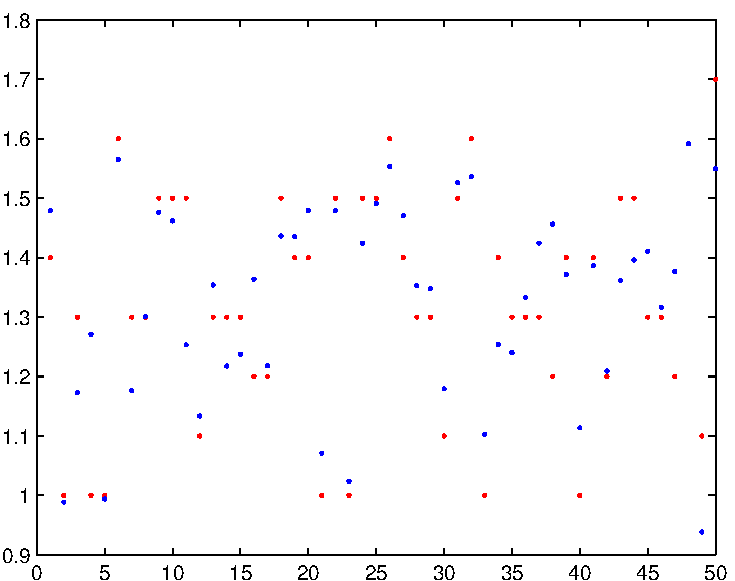
\includegraphics[width=0.4\textwidth]{img/modelolineal_iris}
  \caption{Comparación entre $y$ original e $y$ aproximada}
\end{figure}

Se ve claramente que el uso de este modelo en este caso no es apropiado, porque
la tasa de error es muy alta.

\subsubsection{Conversión al modelo exponencial}

Existen casos en los que el fenómeno observado no se ajuste a un modelo lineal,
para lo que existen otros modelos. El modelo lineal, que hemos usado hasta
ahora, se ajusta a la ecuación:

\[
y = b + a \cdot x
\]

Por otro lado, el \textbf{modelo exponencial} se ajusta a la ecuación:

\[
y = b \cdot e ^{a\cdot x}
\]

Es posible \textbf{convertir} el modelo lineal en el exponencial usando el
logaritmo en base $e$:

\[
y = b \cdot e^{a \cdot x} \Rightarrow \underbrace{log_e \; y}_{y^*} = \underbrace{log_e \; b}_{b^*} + a \cdot x
\]

Internamente:

\[
A =
\begin{bmatrix}
\uparrow & \uparrow \\
x & 1 \\
\downarrow & \downarrow  
\end{bmatrix}, 
\;\; b^* =
\begin{bmatrix}
\uparrow \\
log_e \; y \\
\downarrow  
\end{bmatrix}
\]

Y, tras calcular los coeficientes, deshacer el cambio de
variables para obtener los coeficientes $a$ y $b^*$, usando:

\[
b = e^{b^*} = exp(sol(2))
\]

\textbf{OJO:} recordar el renombramiento de variables.

\paragraph{Ejemplo}

Para el siguiente conjunto de datos:

\begin{figure}[h!]
  \centering
  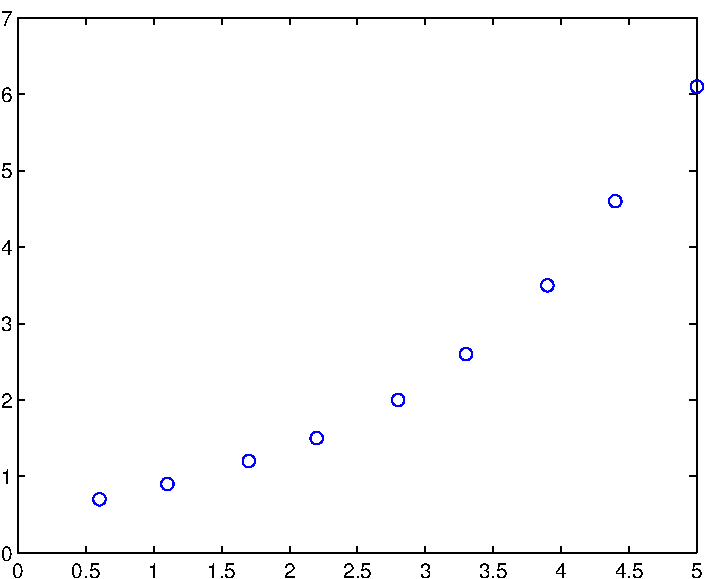
\includegraphics[width=0.4\textwidth]{img/modeloexponencial_1}
\end{figure}

Se ve claramente que los datos no se ajustarían bien a un modelo lineal. Vamos a
hacer el cálculo para un modelo exponencial.

\begin{matlabcode}
% Formato columna
x=[0 0.6 1.1 1.7 2.2 2.8 3.3 3.9 4.4 5]';
y=[0.5 0.7 0.9 1.2 1.5 2 2.6 3.5 4.6 6.1]';

A = [x ones(size(x))];  

% Construimos A con X y la columna de unos
A = [x ones(size(x))];

% B* es el logaritmo de y
b_estrella = log(y);

% La solucion se saca con la formula
sol = pinv(A) * b_estrella;

% El primer elemento es el primer coeficiente
a = sol(1);

% El segundo elemento es b*, por lo que elevamos e a ese elemento
b = exp(sol(2));

% Hacemos la aproximacion
ex = 0:0.1:5;
new_y = b * exp(a*ex)

\end{matlabcode}

\subsubsection{Conversión al modelo polinómico}

Es posible utilizar un modelo lineal para realizar un ajuste a un modelo
polinómico, por ejemplo para un conjunto de datos como el siguiente:

\begin{figure}[h!]
  \centering
  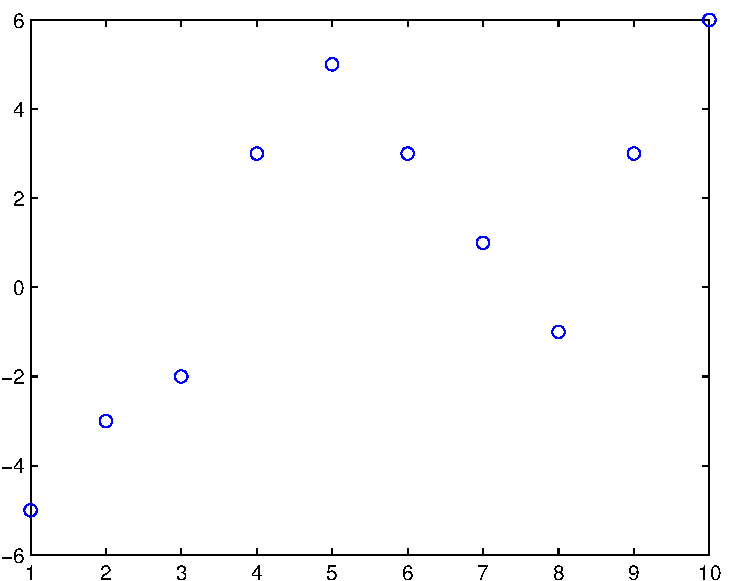
\includegraphics[width=0.4\textwidth]{img/modelopolinomico_1}
\end{figure}

Para ello, usaremos el truco de que dentro del modelo lineal vamos a encontrar
otro modelo lineal con varias entradas. Por ejemplo, para un ajuste
\textbf{cúbico}, que tiene una ecuación \textbf{similar} (que no igual) a:

\[
y = a_3 \cdot x_3 + a_2 \cdot x_2 + a_1 \cdot x_1 + a_o
\]

Nuestro modelo lineal tendrá la siguiente forma:

\[
A =
\begin{bmatrix}
\uparrow & \uparrow & \uparrow & \uparrow\\
x^3 & x^2 & x & 1 \\
\downarrow & \downarrow & \downarrow & \downarrow \\
\end{bmatrix}, 
\;\; b^* =
\begin{bmatrix}
\uparrow \\
y \\
\downarrow  
\end{bmatrix}
\]

Con esto, al resolver el modelo lineal, obtendremos los coeficientes del
polinomio. En Matlab:

\begin{matlabcode}
% Definimos los puntos (en forma de columnas)
x = [1:10]';
y = [-5 -3 -2  3 5 3 1 -1 3 6]';

% Construimos A y b
A = [x.^3 x.^2 x ones(size(x))];
b = y;

% Generamos los coeficientes
sol = pinv(A)*b;

% Esto coincide con el resultado de polyfit(x,y,3)  
\end{matlabcode}

\subsubsection{TO-DO: Conversión para la transformada de Fourier}

\subsubsection{Conversión a otros modelos}

En general, las conversiones de otros modelos al modelo lineal son similares en
tanto en cuanto siempre hay que llegar a una ecuación de la forma

\[
y = b + a \cdot x
\]

\paragraph{Ejemplo 1}

Supongamos una serie de puntos $<x, y>$ que siguen una función de la forma 

\[
y = C \cdot x \cdot e^{A \cdot x}
\]

Dado que hay una exponenciación, lo más adecuado es tomar logaritmos:

\[
log(y) = log(C) + log(x) + A \cdot x
\]

Reordenamos parámetros:

\[
log (y)  - log (x) = A \cdot x + log (C)
\]

Unificamos el lado izquierdo:

\[
log(\frac{y}{x}) = A \cdot x + log(C)
\]

En Matlab:

\begin{matlabcode}
clear all
close all
clc;

x = 1:0.1:10;
y = 4.2 .* x .* exp(2.7 .* x);

% Cambio de variable en los datos
yp = log(y'./x');

aa = [x' ones(size(x'))];
sol = pinv(aa) * yp;

% Regenero los coeficientes originales
A = sol(1); 
C = exp(sol(2));

% Dibujo los puntos originales y el modelo estimado
plot (x, y, 'o'); hold on; axis auto;
xr = 0:0.01:10;
plot(xr, C.*xr.*exp((A)*xr), 'r'); hold off;  
\end{matlabcode}

\paragraph{Ejemplo 2}

Supongamos una serie de puntos $<x, y>$ que queremos ajustar a un modelo con la
siguiente ecuación:

\[
y = a \cdot x^b
\]

Para facilitar las cosas, intercambiamos los nombres de $a$ y $b$:

\[
y = b \cdot x^a
\]

Operamos tomando logaritmos:

\[
log(y) = log(b) + log(x^a) \Rightarrow log(y) = log(b) + a \cdot log(x)
\]

Una vez que tenemos la ecuación en esta forma, operamos con la pseudoinversa y
deshacemos el cambio de variable.

En Matlab:

\begin{matlabcode}
close all
clear all
% clc;

x = [28 50 70];
y = [75 47 34];

yp = log(y');

A = [ log(x)' ones(size(x')) ];
sol = pinv(A) * yp;

a = (sol(1));
b = exp(sol(2));

plot(x, y,'o'); hold on;
xr = 20:75;
yr = b .* xr .^ a;
plot(xr, yr, 'r'); hold off;  
\end{matlabcode}


\subsubsection{Anexo: derivadas habituales}
\label{sec:derivadas_columna}

Sean $z$ y $M$ matrices tales que:

$$
z_{n \times 1} = 
\begin{bmatrix}
z_1 \\
z_2 \\
\vdots \\
z_n
\end{bmatrix},
\;
M_{n \times k} =
\begin{bmatrix}
m_{11} & m_{12} & \dots & m_{1k} \\
m_{21} & m_{22} & \dots & m_{2k} \\
\vdots & \vdots & \ddots & \vdots \\
m_{n1} & m_{n2} & \dots & m_{nk} \\
\end{bmatrix}
$$

Se cumplen las dos siguientes identidades:

\paragraph{Primera identidad}

$$
\frac{\partial z^t M}{\partial z} = M
$$

\begin{proof}
  En efecto, tenemos que:

\[
z^t_{1 \times n} \cdot M_{n \times k} = P_{1 \times k} = \Big[
z_1 \cdot m_{11} + z_2 \cdot m_{21} + \dots + z_n \cdot m_{n1} 
\;\; , \;\; \dots \;\; , \;\;
z_1 \cdot m_{1k} + z_2 \cdot m_{2k} + \dots + z_n \cdot m_{nk} \Big]
\]

La derivada se expande como:

\[
\frac{\partial z^t M}{\partial z} = \frac{\partial P}{\partial z} =
\begin{bmatrix}
\frac{\partial P}{\partial z_1}  \\
\frac{\partial P}{\partial z_2}  \\
\vdots \\
\frac{\partial P}{\partial z_n}
\end{bmatrix}
=
\begin{bmatrix}
\frac{\partial P_1}{\partial z_1} & \frac{\partial P_2}{\partial z_1} & \dots & \frac{\partial P_k}{\partial z_1} \\
\frac{\partial P_1}{\partial z_2} & \frac{\partial P_2}{\partial z_2} & \dots & \frac{\partial P_k}{\partial z_2} \\
\vdots & \vdots & \ddots & \vdots \\
\frac{\partial P_1}{\partial z_n} & \frac{\partial P_2}{\partial z_n} & \dots & \frac{\partial P_k}{\partial z_n}
\end{bmatrix}
\]

Con esto, sabiendo que, por ejemplo:

\[
\frac{\partial P_1}{\partial z_1} = 
\frac{\partial \Big[ z_1 \cdot m_{11} + z_2 \cdot m_{21} + \dots + z_n \cdot m_{n1} \Big]}{\partial z_1} = m_{11}
\]

Se da pues la igualdad:

\[
\frac{\partial z^t M}{\partial z}
=
\begin{bmatrix}
\frac{\partial P_1}{\partial z_1} & \frac{\partial P_2}{\partial z_1} & \dots & \frac{\partial P_k}{\partial z_1} \\
\frac{\partial P_1}{\partial z_2} & \frac{\partial P_2}{\partial z_2} & \dots & \frac{\partial P_k}{\partial z_2} \\
\vdots & \vdots & \ddots & \vdots \\
\frac{\partial P_1}{\partial z_n} & \frac{\partial P_2}{\partial z_n} & \dots & \frac{\partial P_k}{\partial z_n}
\end{bmatrix}
=
\begin{bmatrix}
m_{11} & m_{12} & \dots & m_{1k} \\
m_{21} & m_{22} & \dots & m_{2k} \\
\vdots & \vdots & \ddots & \vdots \\
m_{n1} & m_{n2} & \dots & m_{nk} \\
\end{bmatrix}
=
M
\]

\end{proof}

\paragraph{Segunda identidad}

$$
\frac{\partial z^t M z}{\partial z} = (M + M^t) \cdot z
$$

\begin{proof}

El producto tiene las siguientes dimensiones:
\[
z^t_{1 \times n} \cdot M_{n \times n} \cdot z_{n \times 1} = \square_{1 \times 1}
\]

Por el producto de matrices sabemos que:

\[
z^t M z = \sum_{j=1}^n \sum_{i=1}^n M_{ij} \cdot z_i \cdot z_j
\]

La derivada para un índice $k$ de $z$ sería:

\[
\frac{\partial z^t M z}{\partial z_k} = \frac{\partial}{\partial z_k} \sum_{j=1}^n \sum_{i=1}^n M_{ij} \cdot z_i \cdot z_j =
\sum_{i=1}^n M_{ik} \cdot z_i + M_{ki} \cdot z_i = \sum_{i=1}^n ( M_{ik} + M_{ki} ) \cdot z_i
\]

Generalizando:

\[
\frac{\partial z^t M z}{\partial z} =
\begin{bmatrix}
  \sum_{i=1}^n ( M_{i1} + M_{1i} ) \cdot z_i \\
  \sum_{i=1}^n ( M_{i2} + M_{2i} ) \cdot z_i \\
  \vdots \\
  \sum_{i=1}^n ( M_{in} + M_{ni} ) \cdot z_i
\end{bmatrix}
=
\begin{bmatrix}
  (M_{11} + M_{11}) \cdot z_1 + (M_{21} + M_{12}) \cdot z_2 + \dots \\
  (M_{12} + M_{21}) \cdot z_1 + (M_{22} + M_{22}) \cdot z_2 + \dots \\
  \vdots \\
  (M_{1n} + M_{n1}) \cdot z_1 + (M_{2n} + M_{n2}) \cdot z_2 + \dots 
\end{bmatrix}
=
(M + M^t) \cdot z
\]


% Haciendo la primera parte del producto obtenemos:

% \[
% z^t_{1 \times n} \cdot M_{n \times k} = P_{1 \times k} = \Big[
% z_1 \cdot m_{11} + z_2 \cdot m_{21} + \dots + z_n \cdot m_{n1} 
% \;\; , \;\; \dots \;\; , \;\;
% z_1 \cdot m_{1k} + z_2 \cdot m_{2k} + \dots + z_n \cdot m_{nk} \Big]
% \]

% Si seguimos multiplicando obtenemos:

% \begin{gather*}
% z^t \cdot M \cdot z = \\
% \Big[
% z_1(z_1 \cdot m_{11} + z_2 \cdot m_{21} + \dots + z_n \cdot m_{n1}) 
% + \dots + 
% z_n(z_1 \cdot m_{1k} + z_2 \cdot m_{2k} + \dots + z_n \cdot m_{nk}) \Big]= \\
% \Big[
% z_1^2 \cdot m_{11} + z_1 \cdot z_2 \cdot m_{21} + \dots + z_1 \cdot z_n \cdot m_{n1} 
% + \dots + 
% z_n \cdot z_1 \cdot m_{1k} + z_n \cdot z_2 \cdot m_{2k} + \dots + z_n^2 \cdot m_{nk} \Big]
% \end{gather*}

% Ahora, la derivada respecto de $z$ será un vector columna con las derivadas
% respecto de $z_1$, $z_2$, hasta $z_n$.

% \[
% \frac{\partial z^t M z}{\partial z} =
% \begin{bmatrix}
% \frac{\partial \dots}{\partial z_1} \\
% \frac{\partial \dots}{\partial z_2} \\
% \vdots \\
% \frac{\partial \dots}{\partial z_n} 
% \end{bmatrix}
% =
% \begin{bmatrix}
% 2 \cdot z_1 \cdot m_{11} + z_2 \cdot m_{21} + \dots   
% \end{bmatrix}
% \]


% Aplicando la regla de la derivada de un producto ($ f(x) = u \cdot
%   v \Longrightarrow f'(x) = u' \cdot v + u \cdot v'$) tenemos que:

% \begin{align*}
% \frac{\partial z^t M z}{\partial z} &= \frac{\partial z^t M}{\partial z} \cdot z + z^t M \cdot \overbrace{\frac{\partial z}{\partial z}}^{1}    \\
% &= \frac{\partial z^t M}{\partial z} \cdot z + z^t M
% \end{align*}



% De la demostración de la \textit{primera identidad} sabemos que :

% \[
% \frac{\partial z^t M}{\partial z} = M
% \]

% Lo cual es aplicable al primer término:
% \[
% \frac{\partial z^t M}{\partial z} \cdot z + z^t \cdot M = M \cdot z + z^t \cdot M
% \]

% Si aplicamos la igualdad $A \cdot B = B^t \cdot A^t$ obtenemos:
% \[
% M \cdot z + z^t \cdot M = M \cdot z + M^t \cdot z
% \]

% Y factorizando:
% \[
% \frac{\partial z^t M z}{\partial z} = M \cdot z + M^t \cdot z = (M + M^t) \cdot z
% \]

\end{proof}

\section{Preprocesado}

\subsection{Normalización}

A la hora de trabajar con datos de diferentes tipos en un mismo problema,
conviene \textbf{normalizar} sus valores, de forma que aunque tengan valores muy
dispares, al normalizar los rangos sean similares y los diferentes métodos de
cálculo, como la distancia euclídea, les den la misma importancia.

Con los datos \textbf{ordinales}, lo habitual es mapear los valores en el rango
$[0, 1]$, de forma que el menor valor posible sea 0 y el mayor posible sea 1.

Con los datos \textbf{nominales} (como \textit{blanco}, \textit{rojo}, etc...)
el problema de asignar números es que se introduce una relación implícita que es
incorrecta. Por ejemplo, si a los colores les asignamos números, aquellos con
números cercanos \textbf{tendrían cierta similitud} de cara al sistema, cuando
realmente no es así. Para esos casos se suele calcular el número máximo $N$ de
valores discretos, y disponer $N$ características:

\begin{center}
  \begin{tabular}{r|c|c|c|c}
    blanco & 1 & 0 & 0 & 0 \\ \hline
    rojo   & 0 & 1 & 0 & 0 \\ \hline
    azul   & 0 & 0 & 1 & 0 \\ \hline
    violeta & 0 & 0 & 0 & 1
  \end{tabular}
\end{center}


De esta forma, la distancia euclídea será la misma entre todos los valores.

Para el resto de \textbf{casos especiales} es bueno estudiarlos detenidamente de
forma individualizada, para ver qué técnicas pueden ser interesantes de aplicar.

\subsection{Reducción de la dimensionalidad}

A medida que aumentamos el \textbf{número de características} de los patrones,
va aumentando la \textbf{dimensionalidad} del problema. Es importante tener el
mayor número de patrones y la mayor información posible, pero siempre dentro de
una dimensionalidad adecuada.

Según aumenta la dimensionalidad, los datos van dispersándose más. Por ejemplo,
supongamos el siguiente ejemplo con 100 datos en una sola dimensión:

\begin{figure}[h!]
  \centering
  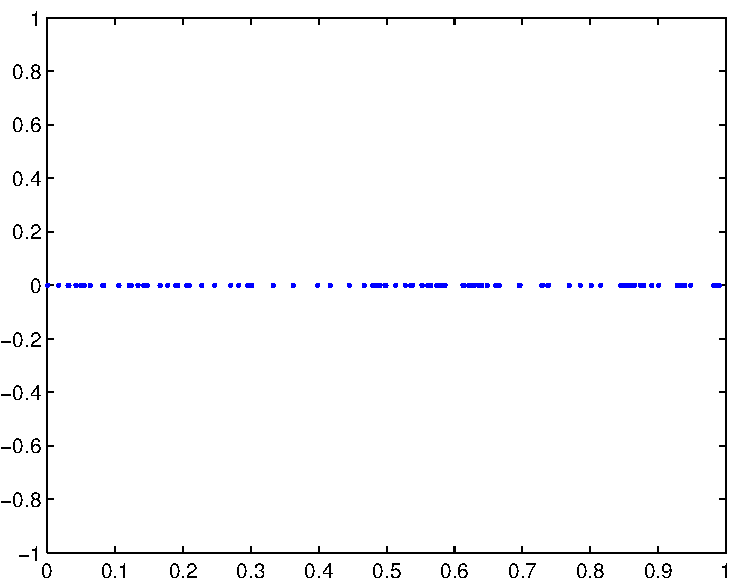
\includegraphics[width=0.5\textwidth]{img/dimensionalidad_1}
\end{figure}

Se ve que la densidad de datos es bastante alta en todo el dominio. Ahora, si
añadimos una segunda dimensión al problema:

\begin{figure}[h!]
  \centering
  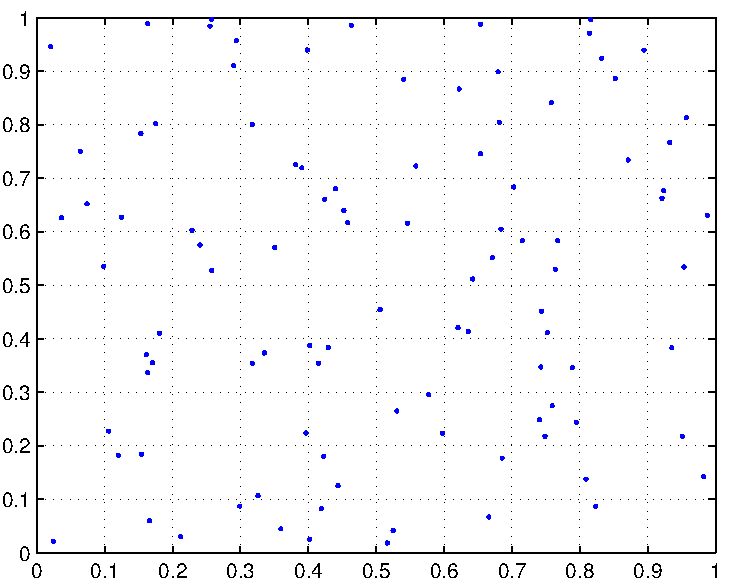
\includegraphics[width=0.5\textwidth]{img/dimensionalidad_2}
\end{figure}

Empezamos a ver zonas que están vacías, que no tienen datos. Según vamos
aumentando la dimensionalidad, los datos se dispersan. Es por ello \textbf{muy
  importante} mantener reducidas las dimensiones del problema.


\subsubsection{Reducción exhaustiva}

Una manera de reducir la dimensionalidad es buscar \textbf{de forma exhaustiva}
las mejores características de entre las originales. Habría que comparar cada
par de características, viendo cuál es más importante.

El problema es que con muchas características el proceso se hace muy
\textbf{tedioso}. Una alternativa es ir añadiendo o reduciendo características y
evaluando los resultados, viendo cómo influyen los cambios.

\subsubsection{Reducción por combinación de características}

La forma más habitual de reducir la dimensionalidad de un problema es
\textbf{combinar características} de forma que, por ejemplo, un problema con 8
dimensiones se reduzca a otro de 2, evitando perder información.

Supongamos que tenemos 8 propiedades $x_1, x_2, \dots, x_8$, y queremos reducir
a 2. Definimos entonces nuevas características $x'$ tales que:

\begin{gather*}
x'_1 = a_1 \cdot x_1 + a_2 \cdot x_2 + \dots + a_8 \cdot x_8 \\  
x'_2 = b_1 \cdot x_1 + b_2 \cdot x_2 + \dots + b_8 \cdot x_8 \\
\vdots
\end{gather*}

Con esto, para $N$ patrones obtendremos un sistema tal que:

\[
x'_{2 \times N} = w_{2 \times 8} \cdot x_{8 \times 1000} \text{ con } w =
\begin{bmatrix}
a_1 & a_2 & \dots & a_8 \\
b_1 & b_2 & \dots & b_8
\end{bmatrix}
\]

Dado que $w$ no es una matriz cuadrada, solo sería posible recuperar una
aproximación $\hat{x}$ a partir de $x'$ y la pseudoinversa de $w$.

\[
x \xRightarrow[]{w} x' \xRightarrow[]{pinv(w)} \hat{x}
\]

El problema, pues, reside en definir bien la matriz $w$ tal que la diferencia
entre $x$ y $\hat{x}$ sea la menor posible.

Los dos métodos más habituales para el cálculo de $w$ son \textbf{PCA} y \textbf{Fisher}.

\subsubsection{Reducción con PCA}

PCA (\textit{análisis de las componentes principales}) es un método clásico para
la reducción de la dimensionalidad que sólo tiene en cuenta los datos de los
patrones, pero no sus clases.

Supongamos que tenemos los siguientes datos en 2 dimensiones que aparecen así en
la gráfica:

\begin{figure}[h!]
  \centering
  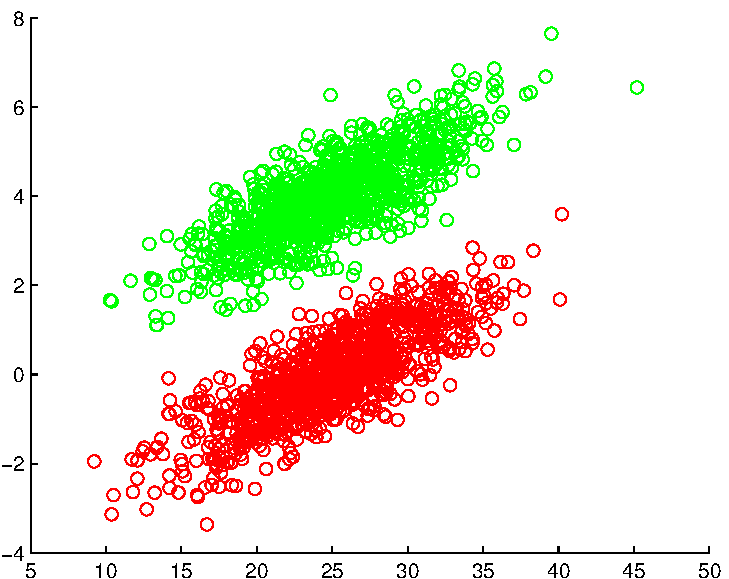
\includegraphics[width=0.5\textwidth]{img/pca_1}
\end{figure}

Si queremos reducir la dimensionalidad a 1, PCA buscaría la dirección en la que
los datos tienen la mayor varianza, y haría la proyección, por ejemplo, sobre
una línea imaginaria como la siguiente:

\begin{figure}[h!]
  \centering
  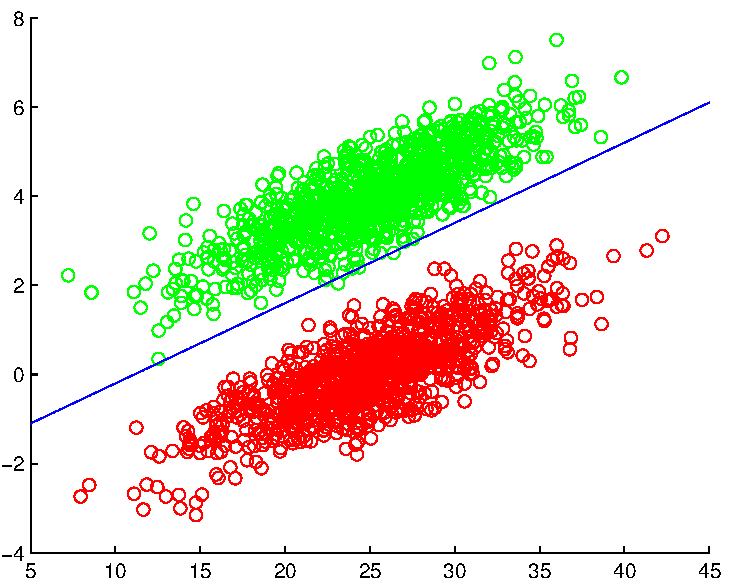
\includegraphics[width=0.5\textwidth]{img/pca_2}
\end{figure}

Lo cual, tras enderezar la proyección a 2 y 1 dimensión, quedaría:

\begin{figure}[h!]
  \centering
  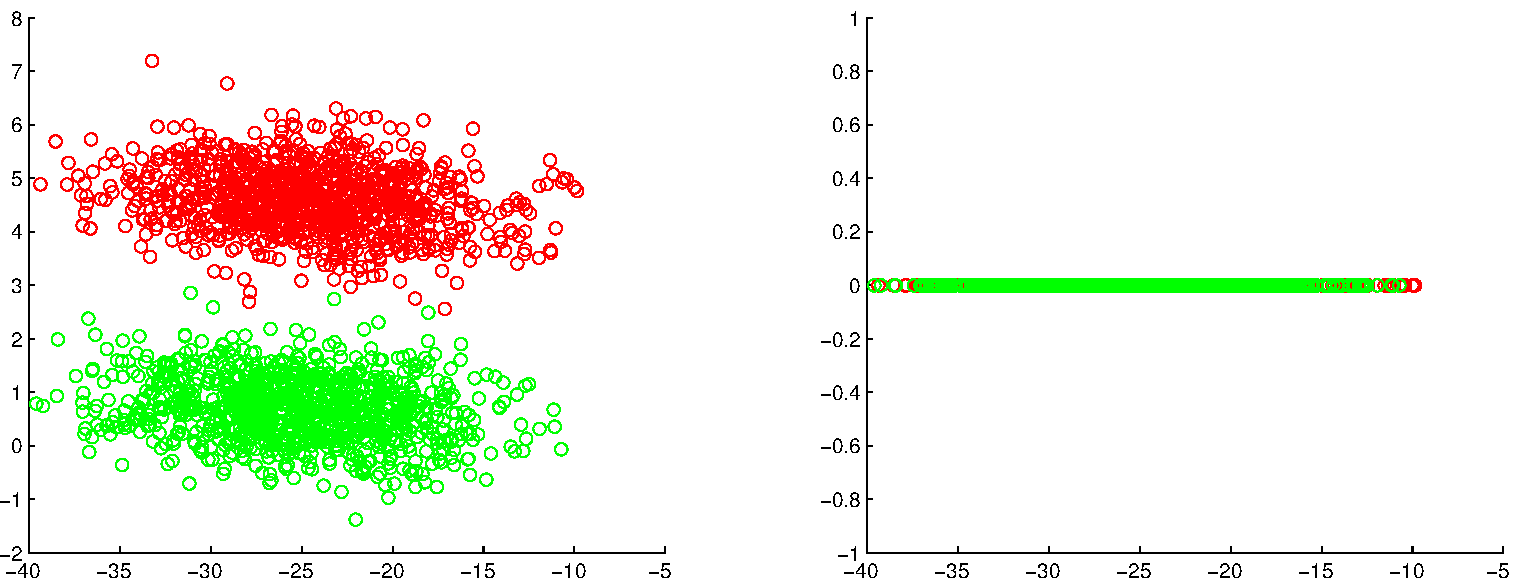
\includegraphics[width=\textwidth]{img/pca_3}
\end{figure}

Como vemos, se produce gran \textbf{confusión}, dado que los datos se mezclan
mucho, dado que no se tiene en cuenta la clasificación.

En Matlab, se haría con la función integrada \texttt{pca}.

\begin{matlabcode}
W = pca(x, 1);

% Proyectamos
xprim = W * x;

% Recuperamos
xgorro = pinv(W) * xprim;
\end{matlabcode}

\subsubsection{Reducción con Fisher}

El método de PCA \textbf{no es adecuado para clasificación}, ya que no tiene en
cuenta las clases de los patrones. En cambio, el \textbf{método de Fisher} sí es
apropiado, ya que consigue que los datos de la misma categoría queden lo más
cerca posible, y que las medias de esas categorías queden lo más separadas
posible.

\begin{figure}[h!]
  \centering
  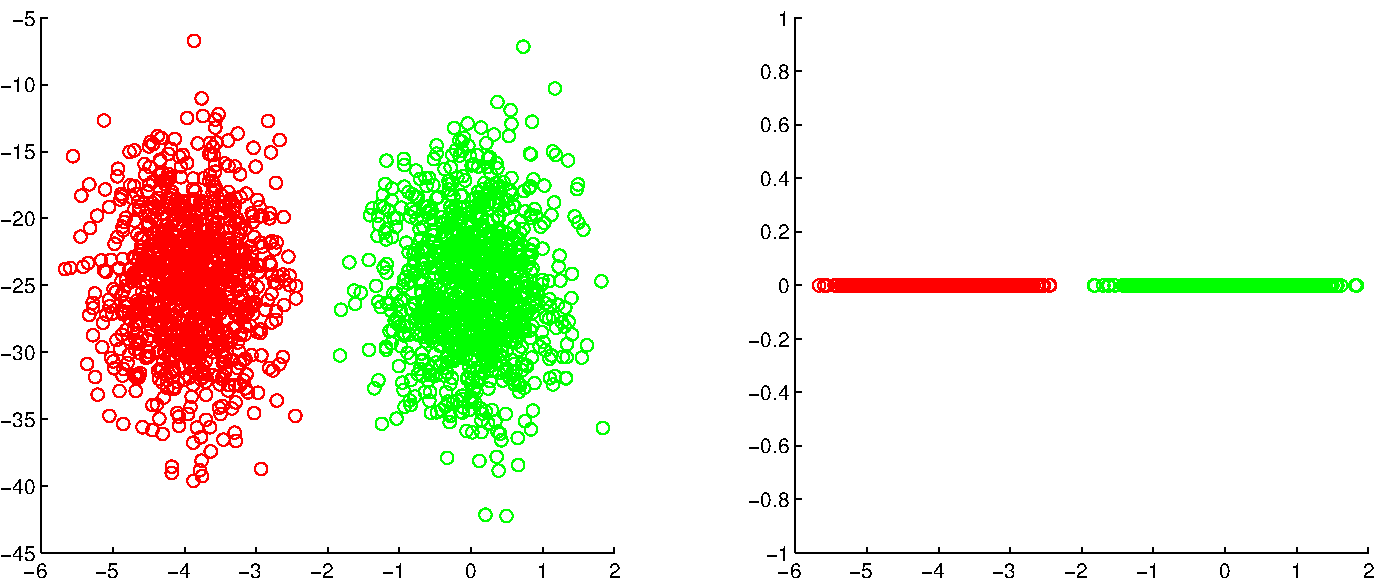
\includegraphics[width=\textwidth]{img/fisher_1}
\end{figure}

En este ejemplo, la proyección de Fisher tendría en cuenta la clasificación de
los datos, y proyectaría de forma que las clases queden muy separadas.

El cálculo en Matlab es similar al de PCA, solo cambiando el método.

\begin{matlabcode}
% Cargamos la BD iris
load iris
y = y + 1;

% Aplicamos fisher para reducir a 2 dimensiones
W = fisher(x,y,2);

% Generamos x prima
xprim = W * x;

% Pintamos x prima
plotpat(xprim, y);
\end{matlabcode}

\pagebreak

\section{Clasificación bayesiana}

\subsection{Introducción}

Supongamos la siguiente población de 100 elementos con la misma probabilidad
$\frac{1}{100}$ de ser elegidos.

\begin{figure}[h!]
  \centering
  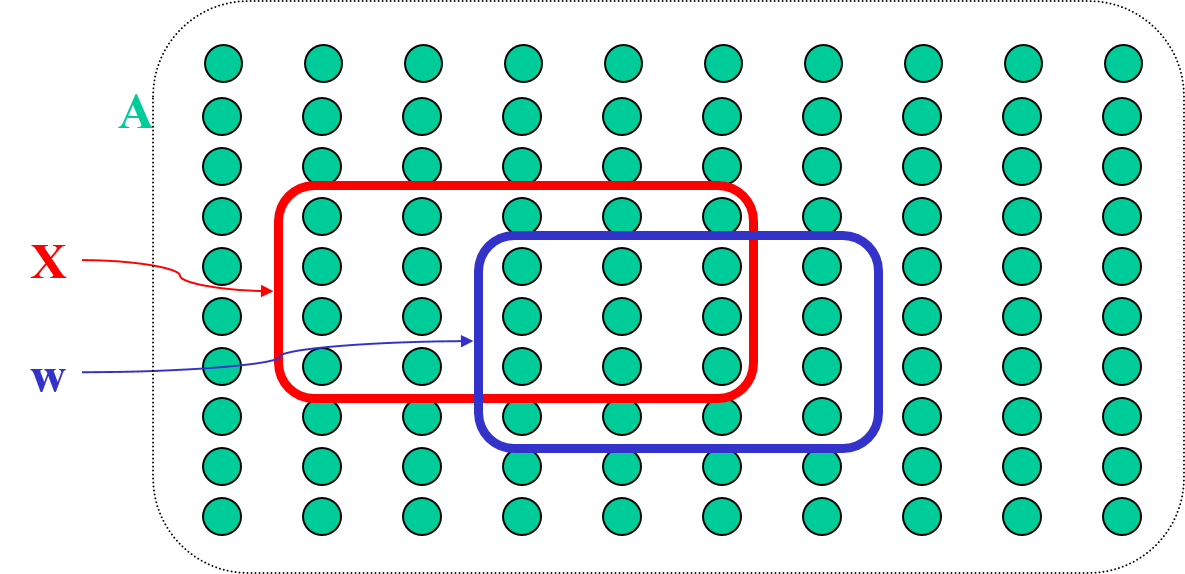
\includegraphics[width=0.7\textwidth]{img/bayes1}
\end{figure}

En el grupo $X$ hay 20 elementos, por lo que la probabilidad de elegir un
elemento de ese grupo de entre el total es $P(X) = \frac{20}{100} = 0.2$.

Por otro lado, en el grupo $W$ hay 16 elementos, por lo que la probabilidad de
elegir un elemento de $W$ es $P(W) = \frac{16}{100} = 0.16$.

Ahora bien, supongamos que queremos conocer la probabilidad de la
\textbf{intersección} de $W$ con $X$, esto es, $w \cap X$. Intuitivamente,
viendo el gráfico sabemos que esa probabilidad es igual a $\frac{9}{100}$.

Numéricamente, la probabilidad de la intersección se puede calcular de dos maneras:

\begin{enumerate}
\item Como la probabilidad de $W$ multiplicada por la probabilidad de
  \textit{que se dé $X$ suponiendo que se ha dado $W$}, lo que se conoce como
  \textbf{probabilidad condicionada}. Es decir, el segundo parámetro supone que
  se da $W$, o lo que es lo mismo, que la población total es $W$, por lo que es
  igual al número de elementos de la población $W$ que también pertenecen a $X$.
\[
P(W \cap X) = P(W) \cdot P(X|W) = \frac{16}{100} \cdot \frac{9}{16} = \frac{9}{100}
\]
\item Como la probabilidad de $X$ multiplicada por la probabilidad de
  \textit{que se dé $W$ suponiendo que se ha dado $X$}. El razonamiento es igual
  al caso anterior:

\[
P(X \cap W) = P(X) \cdot P(W|X) = \frac{20}{100} \cdot \frac{9}{20} = \frac{9}{100}
\]
\end{enumerate}

\subsection{Teorema de Bayes}

El teorema de Bayes se obtiene operando con las anteriores igualdades, y
obteniendo:

\[
P(W|X) = \frac{P(X|W) \cdot P(W)}{P(X)}
\]

\paragraph{Ejemplo}

\begin{figure}[h!]
  \centering
  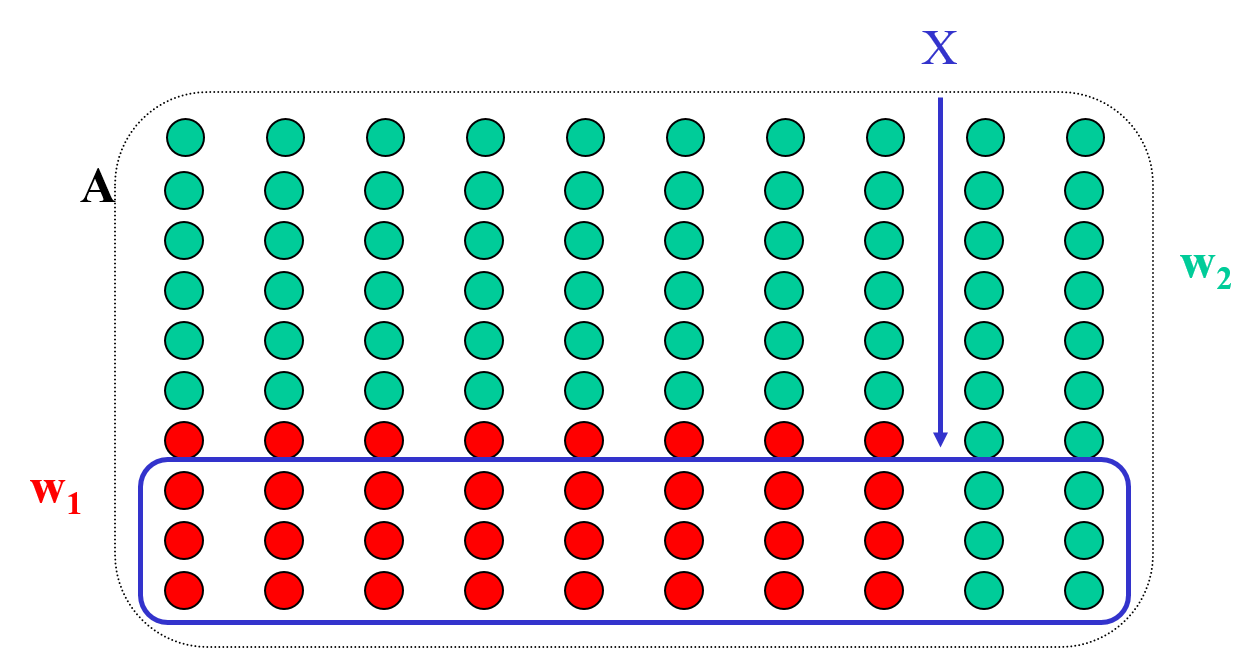
\includegraphics[width=0.7\textwidth]{img/bayes2}
\end{figure}

Supongamos lo siguiente. De los 100 elementos totales,
\begin{itemize}
\item Los 32 elementos rojos son \textbf{mujeres}.
\item Los 68 elementos verdes son \textbf{hombres}.
\item Los 30 elementos dentro del recuadro azul ($X$) son alumnos \textbf{con
    pendiente}. Se ve que \textit{la mayoría} de las chicas tienen pendiente,
  mientras que \textit{la mayoría} de chicos \textbf{no} tienen pendiente.
\end{itemize}

Así, 

\[
P(w1) = \frac{32}{100} ,\;
P(w2) = \frac{68}{100} ,\;
P(X) = \frac{30}{100} 
\]

Si solo tenemos en cuenta la probabilidad de ser hombre o mujer, al elegir un
sujeto aleatoriamente \textit{lo más seguro} es que sea un hombre. Ahora bien,
si del sujeto elegido sabemos una información adicional, que \textbf{tiene
  pendiente}, la cosa cambia, dado que intuitivamente se ve que del grupo de
sujetos con pendiente \textit{lo más seguro} es que sea una mujer.

Visualmente, vemos que las \textbf{probabilidades condicionadas} a que el sujeto
tenga pendientes son:

\begin{gather*}
P(\text{Hombre} | \text{Pendientes}) = \frac{6}{30} \\
P(\text{Mujer} | \text{Pendientes}) = \frac{24}{30} 
\end{gather*}

Ahora, para fundamentar este cálculo podemos usar el teorema de Bayes.

\begin{align*}
P(\text{Hombre} | \text{Pendientes}) &= \frac{P(\text{Pendientes} | \text{Hombre}) \cdot P(\text{Hombre})}{P(\text{Pendientes})} \\
& = \frac{\frac{6}{68} \cdot \frac{68}{100}}{\frac{30}{100}} \\
& = \frac{6}{30}
\end{align*}

El cálculo para el caso de las mujeres es igual. 

\bigskip

\begin{framed}
  
\textbf{Nomenclatura:}
\[
\underbrace{P(W|X)}_\text{Prob. a posteriori} = \frac{\overbrace{P(X|W)}^\text{Prob. condicional} \cdot \overbrace{P(W)}^\text{Prob. a priori}}{P(X)}
\]

La \textbf{nomenclatura} es muy descriptiva. Inicialmente queremos conocer si se
da un hecho $W$, por lo que la probabilidad \textbf{a priori} que tenemos es
$P(W)$. 

Ahora bien, si se da una condición particular ($X$) y sabemos la probabilidad de
que ese hecho ocurra si se da el inicial (la probabilidad \textbf{condicional},
$P(X|W$)), entonces estaremos obtenido la probabilidad \textbf{a posteriori}, es
decir, la probabilidad tras conocer la circunstancia adicional.

\end{framed}

Esto tiene gran utilidad en problemas de \textbf{clasificación}, ya que
conociendo ciertas propiedades (por ejemplo \textit{tiene pendientes} y
\textit{tiene barba}), y sabiendo las probabilidades de entre la población,
puedo saber la probabilidad de que sea de una clase u otra.

A la hora de seleccionar una hipótesis existen dos variantes:

\begin{itemize}
\item \textbf{Criterio MAP (Máximo A-Posteriori)}: consiste en elegir aquella
  hipótesis con la mayor probabilidad \textit{a posteriori}. Normalmente el
  denominador es igual en todas las hipótesis, por lo que se puede
  \textbf{descartar}.
\item \textbf{Criterio Máxima Verosimilitud}: consiste en comparar utilizando
  únicamente la \textbf{probabilidad condicional}, ya que es frecuente tratar
  con clases que tienen la misma probabilidad a priori.
\end{itemize}

\subsection{Funciones de densidad de probabilidad}

Con frecuencia, los valores con los que se trabajan son \textbf{continuos} (por
ejemplo, la \textit{altura} de un grupo de personas). En estos casos, $P(X)$ es
una \textbf{función de densidad de probabilidad}. El área bajo su curva es 1.

\begin{figure}[h!]
  \centering
  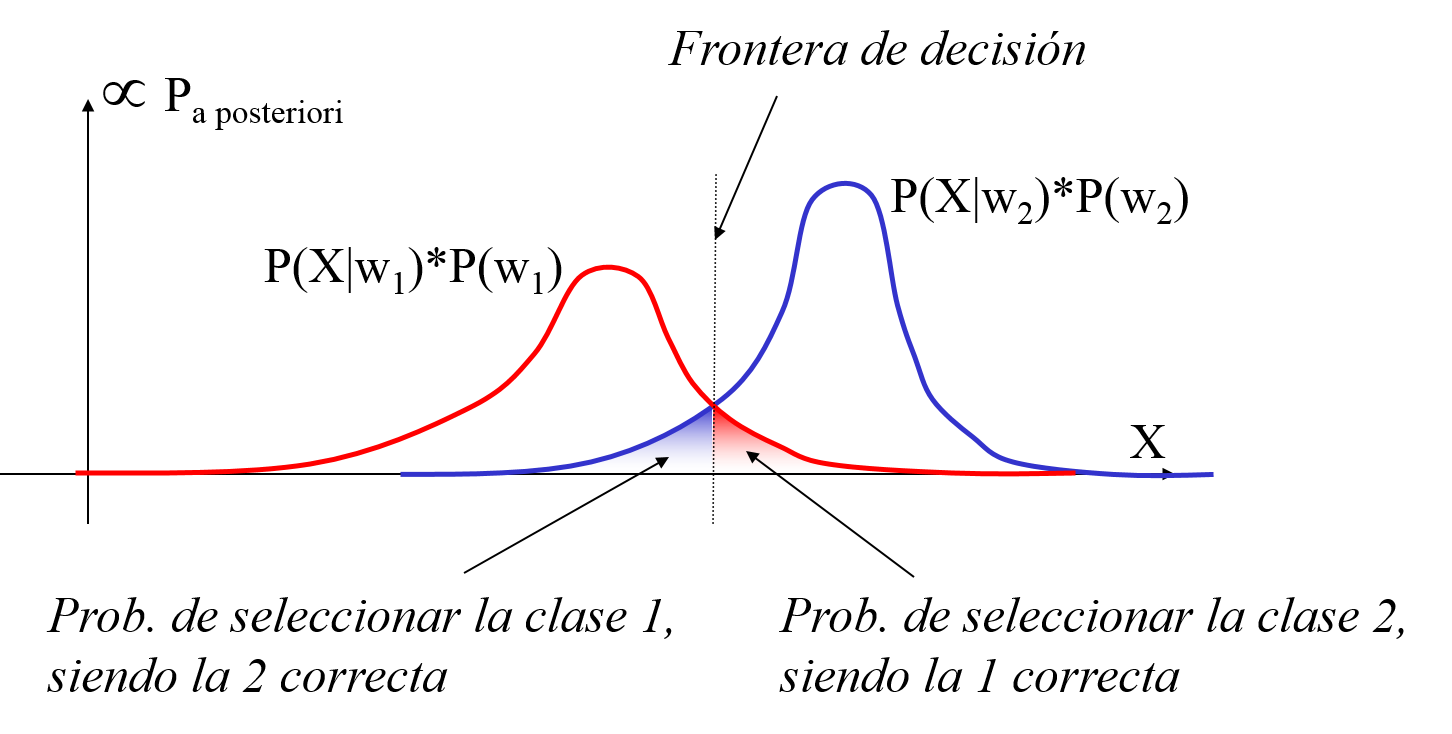
\includegraphics[width=0.9\textwidth]{img/bayes3}
\end{figure}

El problema de decidir la probabilidad a posteriori se ve gráficamente como
decidir la posición de la \textbf{frontera de decisión}. El primer conjunto de
métodos para ello son los \textbf{métodos paramétricos}. 

Suponen que las probabilidades implicadas tienen una forma dada, normalmente una
\textbf{gausiana}. Para modelar las distribuciones de cada conjunto de datos
simplemente se calcula la media y la desviación típica ($\sigma^2$).

\begin{matlabcode}
% Calculamos la media y desv. estandar
media1 = mean(x1);
desv1 = std(x1);

% Podemos generar 1000 datos adicionales de la normal
datos_adicionales = media1 + desv1 * randn(1, 1000);  

% Forma alternativa
datos_adicionales = randnorm(media1, desv1, 1000);

% Forma alternativa indicando el eje de abcisas
X = [0:0.01:30];
Y = normpdf(X, media1, desv1);
\end{matlabcode}

\begin{framed}
En una gausiana, los valores \textbf{se distribuyen así}:

\begin{center}
  \begin{tabularx}{\textwidth}{X X X}
    $\mu \pm \sigma$ & $\mu \pm 2 \cdot \sigma$ & $\mu \pm 3 \cdot \sigma$ \\
    68.27\% & 95.45 \% & 99.73 \%
  \end{tabularx}
\end{center}

\end{framed}

En este caso, la frontera de decisión óptima siempre es aquella en la que las
gausianas cortan, esto es, aquella en la que las gausianas tienen el mismo
valor. Nos basaremos en la definición de la función de densidad de probabilidad gausiana:

\[
\frac{1}{\sqrt{2\pi\sigma^2}}\; e^{ - \frac{(x-\mu)^2}{2 \sigma^2}}
\]

\subsubsection{Cálculo de la frontera con iguales probs. a priori e igual desv. típica}

Suponiendo que las probabilidades a priori son las mismas, el cálculo de la
probabilidad a posteriori se reduce a la probabilidad condicional. Suponemos
también que la desviación típica es igual en ambas distribuciones ($\sigma_1 =
\sigma_2$).

Igualamos:

\[
\frac{1}{\sqrt{2\pi\sigma_1^2}}\; e^{- \frac{(x-\mu_1)^2}{2 \sigma_1^2}} = \frac{1}{\sqrt{2\pi\sigma_2^2}}\; e^{- \frac{(x-\mu_2)^2}{2 \sigma_2^2}}
\]

Como hemos supuesto que $\sigma_1 = \sigma_2 \ne 0$, el coeficiente que
multiplica puede eliminarse de ambos lados:

\[
e^{- \frac{(x-\mu_1)^2}{2 \sigma_1^2}} = e^{- \frac{(x-\mu_2)^2}{2 \sigma_2^2}}
\]

Al tener dos exponenciales, podemos tomar logaritmos y nos quedamos con los
exponentes:

\[
\frac{(x-\mu_1)^2}{2 \cdot \sigma_1^2} = \frac{(x-\mu_2)^2}{2 \cdot \sigma_2^2} 
\]

Igual que antes, factorizamos y eliminamos el coeficiente de $\sigma$:

\[
(x - \mu_1)^2 = (x - \mu_2)^2
\]

Expandimos los binomios al cuadrado

\begin{align*}
x^2 + \mu_1^2 - 2 \cdot x \cdot \mu_1 &= x^2 + \mu_2^2 - 2 \cdot x \cdot \mu_2 \\
\mu_1^2 - 2 \cdot x \cdot \mu_1 &= \mu_2^2 - 2 \cdot x \cdot \mu_2 \\
\mu_1^2 - \mu_2^2 = 2 \cdot x \cdot (\mu_1 - \mu_2)
\end{align*}

Expandimos la parte izquierda por la regla $a^2 - b^2 = (a+b)(a-b)$:

\begin{align*}
(\mu_1 + \mu_2)(\mu_1 - \mu_2) &= 2 \cdot x \cdot (\mu_1 - \mu_2) \\
\mu_1 + \mu_2 &= 2 \cdot x \\
x &= \frac{\mu_1 + \mu_2}{2}
\end{align*}

\begin{framed}
  \begin{wrapfigure}{l}{.3\textwidth}

    \medskip \medskip \medskip

\[
x = \frac{\mu_1 + \mu_2}{2}
\]
\end{wrapfigure}

Así, la frontera óptima estará en esa posición si se cumplen estas
restricciones:
\begin{enumerate}
\item Ambas curvas son normales.
\item Las probabilidades \textit{a priori} son iguales, $P(w_1) = P(w_2)$.
\item Las desviaciones típicas son iguales, $\sigma_1 = \sigma_2$.
\end{enumerate}
\end{framed}

\subsubsection{Cálculo de la frontera óptima para el caso general}
\label{sec:frontera_general}
Para el caso general, la frontera óptima ha de cumplir que:

\[
P(X|w_1) * P(w_1) = P(X|w_2) * P(w_2)
\]

Sacamos logaritmos:

\[
log(\frac{1}{\sqrt{2 \pi \sigma_1^2}}) - \frac{(x - \mu_1)^2}{2 \sigma_1^2} + log(P(w_1)) = log(\frac{1}{\sqrt{2 \pi \sigma_2^2}}) - \frac{(x - \mu_2)^2}{2 \sigma_2^2} + log(P(w_2))
\]

Desarrollamos el primer logaritmo sabiendo que $log (\frac{a}{b}) = log (a) - log (b)$ y que $log (\sqrt{a}) = \frac{1}{2} log (a)$:

\[
log(1) - \frac{1}{2} log(2\pi) - \frac{1}{2} log(\sigma_1^2) - \frac{(x - \mu_1)^2}{2 \sigma_1^2} + log(P(w_1)) = log(1) - \frac{1}{2} log(2\pi) - \frac{1}{2} log(\sigma_2^2) - \frac{(x - \mu_2)^2}{2 \sigma_2^2} + log(P(w_2))
\]

Quitamos de ambos lados las constantes y operamos aplicando $log(a^b) = b \cdot log(a)$:

\[
-log(\sigma_1) - \frac{(x - \mu_1)^2}{2 \cdot \sigma_1^2} + log(P(w_1)) = - log(\sigma_2^2) - \frac{(x - \mu_2)^2}{2 \cdot \sigma_2^2} + log(P(w_2))
\]

Ahora, para quitar las fracciones sacamos común denominador $2 \cdot \sigma_1^2 \cdot \sigma_2^2$:

\begin{gather*}
  - 2 \cdot \sigma_1^2 \cdot \sigma_2^2 \cdot log(\sigma_1) - \sigma_2^2 \cdot ((x-\mu_1)^2) + 2 \cdot \sigma_1^2 \cdot \sigma_2^2 \cdot log(P(w_1)) \\
  = \\
  - 2 \cdot \sigma_1^2 \cdot \sigma_2^2 \cdot log(\sigma_2) - \sigma_1^2 \cdot ((x-\mu_2)^2) + 2 \cdot \sigma_1^2 \cdot \sigma_2^2 \cdot log(P(w_2)) \\
\end{gather*}

Expandimos el binomio central y movemos todo al mismo lado:

\begin{gather*}
  - 2 \cdot \sigma_1^2 \cdot \sigma_2^2 \cdot log(\sigma_1)
  - \sigma_2^2 \cdot x^2 - \sigma_2^2 \cdot \mu_1^2 + 2 \cdot x \cdot \mu_1 \cdot \sigma_2^2 
  + 2 \cdot \sigma_1^2 \cdot \sigma_2^2 \cdot log(P(w_1)) \\
  + 2 \cdot \sigma_1^2 \cdot \sigma_2^2 \cdot log(\sigma_2) 
  + \sigma_1^2 \cdot x^2  - 2 \cdot x \cdot \mu_2 \cdot \sigma_1^2
  - 2 \cdot \sigma_1^2 \cdot \sigma_2^2 \cdot log(P(w_2)) \\
  = 0
\end{gather*}

Ahora, agrupamos según multipliquen a $x^2$, a $x$ o sean términos independientes:

\begin{gather*}
  x^2 \cdot (\sigma_1^2 - \sigma_2^2) + \\
  x   \cdot (2 \cdot \mu_1 \cdot \sigma_2^2  - 2 \cdot \mu_2 \cdot \sigma_1^2) \\
  - 2 \cdot \sigma_1^2 \cdot \sigma_2^2 \cdot log(\sigma_1) - \sigma_2^2 \cdot \mu_1^2 + 2 \cdot \sigma_1^2 \cdot \sigma_2^2 \cdot log(P(w_1)) \\
  + 2 \cdot \sigma_1^2 \cdot \sigma_2^2 \cdot log(\sigma_2) + \sigma_1^2 \cdot \mu_2^2 - 2 \cdot \sigma_1^2 \cdot \sigma_2^2 \cdot log(P(w_2))
\end{gather*}

Factorizamos los términos independientes:

\begin{gather*}
  x^2 \cdot (\sigma_1^2 - \sigma_2^2) + \\
  x   \cdot (2 \cdot \mu_1 \cdot \sigma_2^2  - 2 \cdot \mu_2 \cdot \sigma_1^2) \\
  + 2 \cdot \sigma_1^2 \cdot \sigma_2^2 \cdot \Big[ log(P(w_1)) - log(\sigma_1) - log(P(w_2)) + log(\sigma_2) \Big] \\
  + (\sigma_1^2 \cdot \mu_2^2 - \sigma_2^2 \cdot \mu_1^2)
\end{gather*}

\begin{framed}
  Así, llegamos a una ecuación del tipo $Ax^2 + Bx + C = 0$ donde:

\begin{align*}
  A &= \sigma_1^2 - \sigma_2^2 \\
  B &= 2(\mu_1 \cdot \sigma_2^2 - \mu_2 \cdot \sigma_1^2) \\
  C &= \Big[ ln(P(w_1)) - ln(\sigma_1) - ln(P(w_2)) + ln(\sigma_2) \Big] \cdot 2
  \cdot \sigma_1^2 \cdot \sigma_2^2 + (\sigma_1^2 \cdot \mu_2^2 - \sigma_2^2
  \cdot \mu_1^2)
\end{align*}

\end{framed}

\paragraph{Ejemplo}

En Matlab, suponiendo un conjunto de patrones $X_{1 \times 5000}$ y $Y_{1 \times 5000}$:

\begin{figure}[h!]
  \centering
  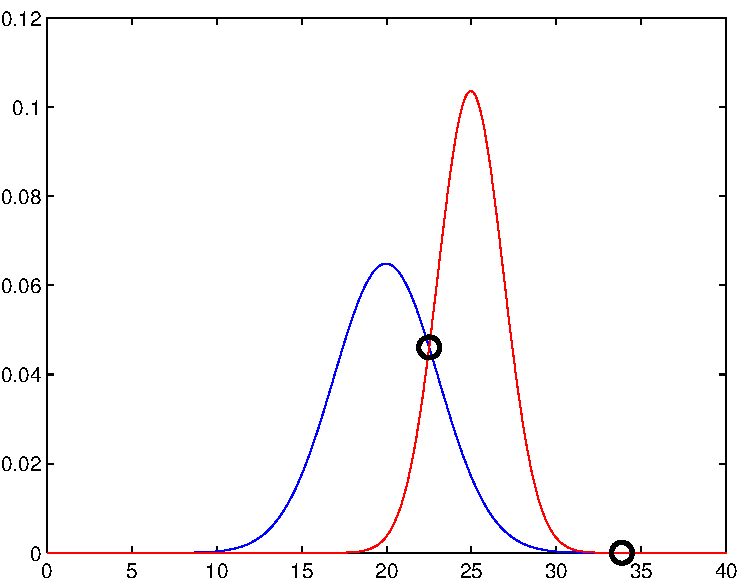
\includegraphics[width=0.5\textwidth]{img/bayes_4}
\end{figure}

\begin{matlabcode}
i1 = find(y == 0);
i2 = find(y == 1);

m1 = mean(x(i1));
m2 = mean(x(i2));

s1 = std(x(i1));
s2 = std(x(i2));

Pw1 = length(i1) / length(y);
Pw2 = length(i2) / length(y);

A=s1*s1-s2*s2;
B=2*(m1*s2*s2-m2*s1*s1);
C=2*s1*s1*s2*s2*(log(Pw1)-log(Pw2)-log(s1)+log(s2))+s1*s1*m2*m2-s2*s2*m1*m1;
x1=(-B+sqrt(B*B-4*A*C))/2/A
x2=(-B-sqrt(B*B-4*A*C))/2/A

I=0:0.01:40;
plot(I,Pw1*normpdf(I,m1,s1));     hold on;
plot(I,Pw2*normpdf(I,m2,s2),'r'); 

plot(x1, Pw1 * normpdf(x1,m1,s1), 'ko', 'LineWidth', 2, 'MarkerSize', 10);
plot(x2, Pw1 * normpdf(x2,m1,s1), 'ko', 'LineWidth', 2, 'MarkerSize', 10);

hold off;  
\end{matlabcode}


\subsection{Distribuciones bidimensionales}

Es posible trabajar en dos dimensiones, los patrones serán vectores columnas con
la forma $\vec{x} = \begin{bmatrix} x_1 \\ x_2 \end{bmatrix}$, por lo que hay
que adaptar la fórmula de la función de densidad de probabilidad:

\[
f_X(x_1, \dots, x_n)=\frac {1} {(2\pi)^{n/2} \left|\Sigma\right|^{1/2}}
\;\; e ^{\left( -\frac{1}{2}( x - \mu)^\top \Sigma^{-1} (x - \mu)\right)}
\]

Donde $\sum$ es la matriz de covarianza. En el caso de dos dimensiones, $n=2$ y 

\[
\vec{x} =
\begin{bmatrix}
  x_1 \\ x_2
\end{bmatrix}
, \vec{\mu} = 
\begin{bmatrix}
  \mu_1 \\ \mu_2
\end{bmatrix}
, \sum =
\begin{bmatrix}
  \sum_{11} & \sum_{12} \\
  \sum_{21} & \sum_{22}
\end{bmatrix}
\]

En Matlab, podemos generar una normal multivariada con mvnpdf
(\textit{multivariate normal probability density function}):

\begin{matlabcode}
[x,y]=meshgrid(-3:0.1:5);

m1 = [0;0];	
C1 = [1 0;0 1];
D1 = mvnpdf([x(:) y(:)], m1',C1);
D1 = reshape(D1,size(x));
mesh(D1), axis vis3d;  
\end{matlabcode}

\begin{figure}[h!]
  \centering
  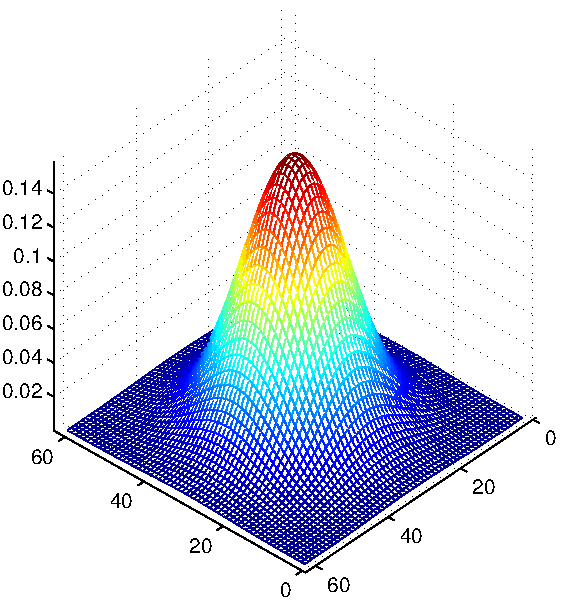
\includegraphics[width=0.6\textwidth]{img/bayes_2d_1}
\end{figure}

También es posible generar los valores con \texttt{randnorm}. Si hacemos un
ploteo en 2 dimensiones es posible pintar la frontera con \texttt{plotbon}. La
intersección de dos gausianas en 2D sigue la forma de una cónica, cuya función
es:

\[
f(x,y) = a x^2 + b y^2 + c x y + d x + e y + f
\]

\subsubsection{Ejemplo, medias diferentes e igual covarianza}

\begin{figure}[h!]
  \centering
  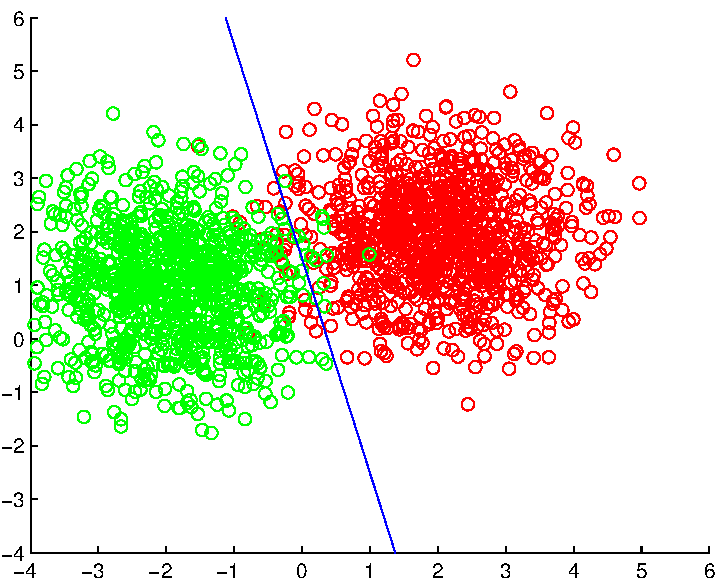
\includegraphics[width=0.6\textwidth]{img/bayes_2d_2}
  \label{Medias diferentes e igual covarianza}
\end{figure}

\begin{matlabcode}
m1=[2;2]; m2=[-2;1]; C1=[1 0;0 1]; C2=[1 0;0 1];
x=[randnorm(m1,C1,1000) randnorm(m2,C2,1000)];
y=[zeros(1,1000) ones(1,1000)];
plotpat(x,y);
hold on;
plotbon(m1,C1,m2,C2,'b');
axis([-4 6 -4 6])  
\end{matlabcode}

\subsubsection{Medias iguales y covarianzas proporcionales}

\begin{figure}[h!]
  \centering
  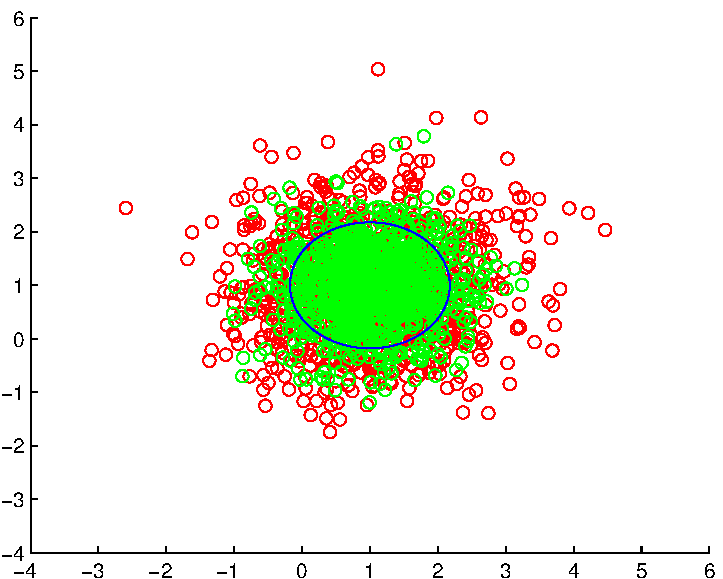
\includegraphics[width=0.6\textwidth]{img/bayes_2d_3}
  \label{Medias iguales y covarianzas proporcionales}
\end{figure}

\begin{matlabcode}
m1=[1;1]; m2=[1;1]; 
C1=[1 0;0 1]; C2=[0.5 0;0 0.5];  
\end{matlabcode}

\subsubsection{Medias iguales y covarianzas diferentes}

\begin{figure}[h!]
  \centering
  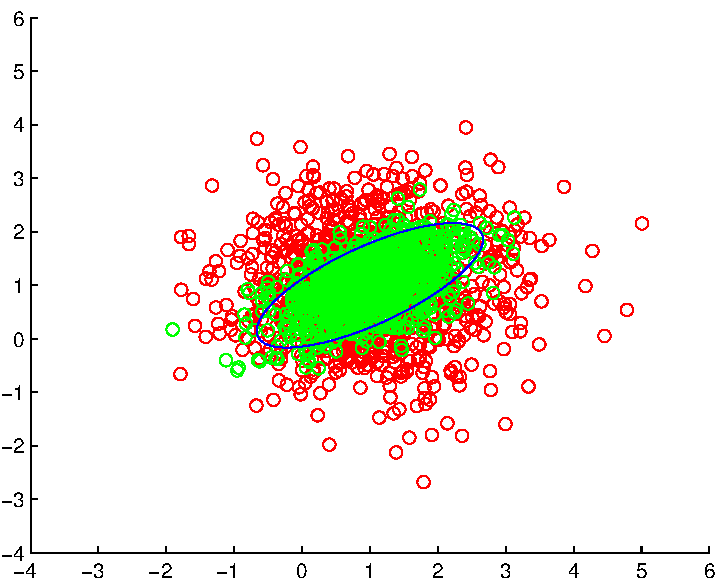
\includegraphics[width=0.6\textwidth]{img/bayes_2d_4}
  \label{Medias iguales y covarianzas proporcionales}
\end{figure}

\begin{matlabcode}
m1=[1;1]; m2=[1;1]; 
C1=[1 0;0 1]; C2=[0.5 0.2;0.2 0.3];  
\end{matlabcode}

\subsubsection{Medias y covarianzas distintas}

\begin{figure}[h!]
  \centering
  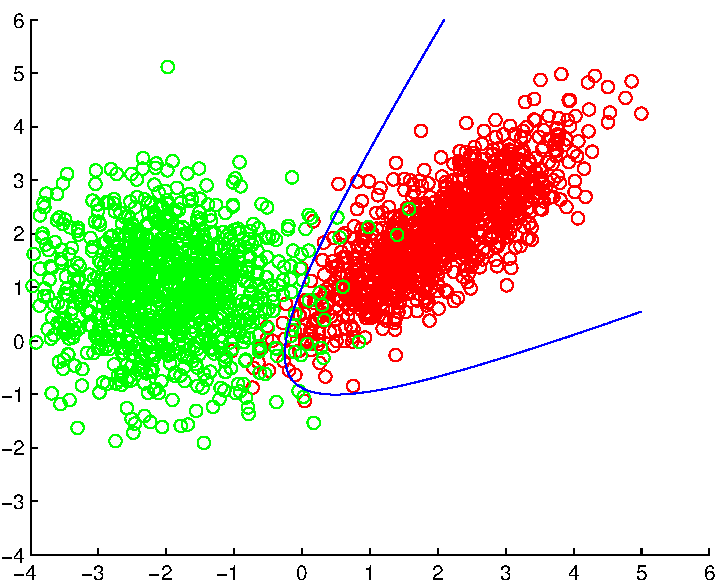
\includegraphics[width=0.6\textwidth]{img/bayes_2d_5}
  \label{Medias iguales y covarianzas proporcionales}
\end{figure}

\begin{matlabcode}
m1=[2;2]; m2=[-2;1]; 
C1=[1 0.8;0.8 1]; C2=[1 0;0 1];  
\end{matlabcode}

\subsection{Toma de decisiones con costes}

Hay ocasiones en las que cometer un error en la clasificación \textbf{es más
  costoso} si un elemento de una clase $A$ se coloca en la clase $B$ que en el
caso contrario.

Por ejemplo, tenemos un sistema de defensa contra misiles que detecta si un
misil ha sido lanzado contra el país y lo destruye con unas contramedidas. Si el
sistema que detecta la amenaza \textbf{clasifica de forma errónea} un misil
real, éste acaba impactando y se producen muchas bajas, por lo que el coste del
error de clasificación es \textbf{alto}.

En cambio, si da un falso positivo y cree que una gaviota es un misil, entonces
el único gasto que se produce es en las contramedidas utilizadas... y en la vida
de la gaviota. Por tanto, el coste del error es \textbf{bajo}.

Así, es preferible que el sistema sea más sensible a las amenazas, por el coste
de un error u otro.

En estos casos se utiliza una \textbf{matriz de costes}, en la que se resume el
coste de los aciertos y los errores: el elemento $L_{ij}$ es el coste de elegir
la clase $j$ cuando la clase real es la $i$.

\begin{center}
  \begin{tabular}[h!]{c c|c|c}
    &         & \multicolumn{2}{c}{Predicción} \\ \cline{2-4}
    & $L_{ij}$ & 1 & 2 \\ \hline
    \multirow{2}{*}{
      \begin{sideways}
        Real
      \end{sideways}
    } & 1 & $10^2$ & $10^4$ \\ \cline{2-4}
    & 2 & $10^6$ & $10^4$ 
  \end{tabular}
\end{center}


\subsubsection{Riesgo de predicción}

Es posible estimar la pérdida general por errores de clasificación utilizando el
teorema de Bayes, lo cual da lugar a la expresión del \textbf{riesgo de
  predicción}, donde $M$ es el número de clases existentes:

\[
r_j(x) = \sum_{i=1}^M L_{ij} \cdot P(x|w_i) \cdot P(w_i)
\]

\subsubsection{Aplicación gausiana}

A la hora de aplicar la matriz de costes cuando trabajemos con distribuciones
gausianas, tenemos dos opciones:

\begin{itemize}
\item Aplicarle el coste al cálculo del histograma: $$hist \cdot L_{ij}$$

\item Aplicarle el coste a la expresión de la probabilidad: 
\[
L_{12} \cdot P(X|w_1) \cdot P(w_1)
\]
\end{itemize}

Esto hace que la frontera \textbf{se mueva} hacia la dirección en la que es más
barato el error. El cálculo formal de la frontera se reduce a resolver la ecuación:

\[
P(X|w_1) \cdot P(w_1) \cdot L_{12} = P(X|w_2) \cdot P(w_2) \cdot L_{21}
\]

La demostración es básicamente igual a la que se expone en la sección
\textit{\nameref{sec:frontera_general}}, con la única diferencia de que los dos
nuevos parámetros pasan al final a formar parte del término independiente del
polinomio resultante, quedando así los coeficientes:

\begin{align*}
  A &= \sigma_1^2 - \sigma_2^2 \\
  B &= 2(\mu_1 \cdot \sigma_2^2 - \mu_2 \cdot \sigma_1^2) \\
  C &= \Big[ ln(L1) - ln(L2) +  ln(P(w_1)) - ln(\sigma_1) - ln(P(w_2)) + ln(\sigma_2) \Big] \cdot 2 \cdot \sigma_1^2 \cdot \sigma_2^2 + (\sigma_1^2 \cdot \mu_2^2 - \sigma_2^2 \cdot \mu_1^2)
\end{align*}

\subsection{Ventanas de Parzen}

Hay ocasiones en las que la distribución subyacente de los datos no es una
normal, por lo que los métodos que conocemos no funcionan bien. El método de las
\textbf{ventanas de Parzen} generan una distribución conjunta de muchas
distribuciones individuales \textbf{centradas en cada dato}, que se suman y
normalizan a área 1 dividiendo entre el número de datos. Habitualmente se
utiliza con \textbf{gausianas}.

\begin{figure}[h!]
  \centering
  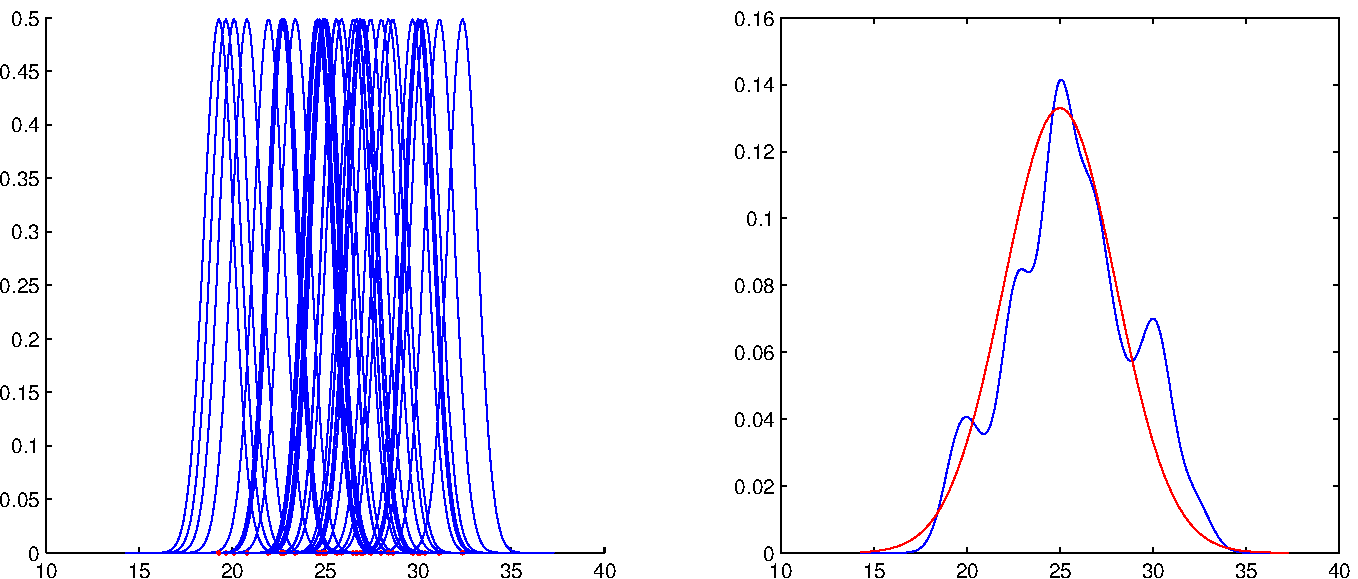
\includegraphics[width=0.8\textwidth]{img/parzen_1}
  \caption{Distribuciones individuales y sumadas. Se han usado 20 datos de una $N(0,1)$.}
\end{figure}

La \textbf{desviación típica} de las gausianas, que controla su amplitud, se
determinará atendiendo a diferentes criterios, como el número de puntos o la
separación entre ellos. Si usamos una $\sigma$ demasiado grande, se achatará
mucho el resultado, \textbf{suavizando demasiado} los detalles. En cambio, si
usamos una $\sigma$ demasiado pequeña, habrá muchos picos. Es habitual utilizar
un bucle para decidirse por el valor de $\sigma$ que menor error dé.

\begin{matlabcode}
datos=shuffle([randn(1,1000)*5+30 randn(1,1000)*3+17]);
desvstandard=0.75;
x=5:0.1:45;
h=zeros(1,length(x));
for i=1:length(datos),  
  t = normpdf(x,datos(i), desvstandard);
  h = h + t;  

  plot(x, t);  hold on;
end 

h = h / length(datos);
h2 = (normpdf(x,30,5) + normpdf(x,17,3))/2;

figure, plot(x,h,'r',x,h2,'b');
legend('calculada','exacta')
\end{matlabcode}

\subsubsection{Diferentes distribuciones}

El procedimiento de las ventanas de Parzen no solo funciona con distribuciones
gausianas, sino que es posible usar otras clases de distribuciones para estimar
la función de densidad subyacente. Por ejemplo, es posible utilizar la función
de densidad \textbf{uniforme} que, centrada en un punto $M$ y usando un ancho
$T$, asigna la misma densidad a los elementos en el rango $[M - \frac{T}{2}, M +
\frac{T}{2}]$, y 0 a los elementos fuera de ese rango. Es una especie de función
\textbf{escalón}. En este caso, el parámetro que habrá que optimizar será el
\textbf{ancho}.

\begin{figure}[h!]
  \centering
  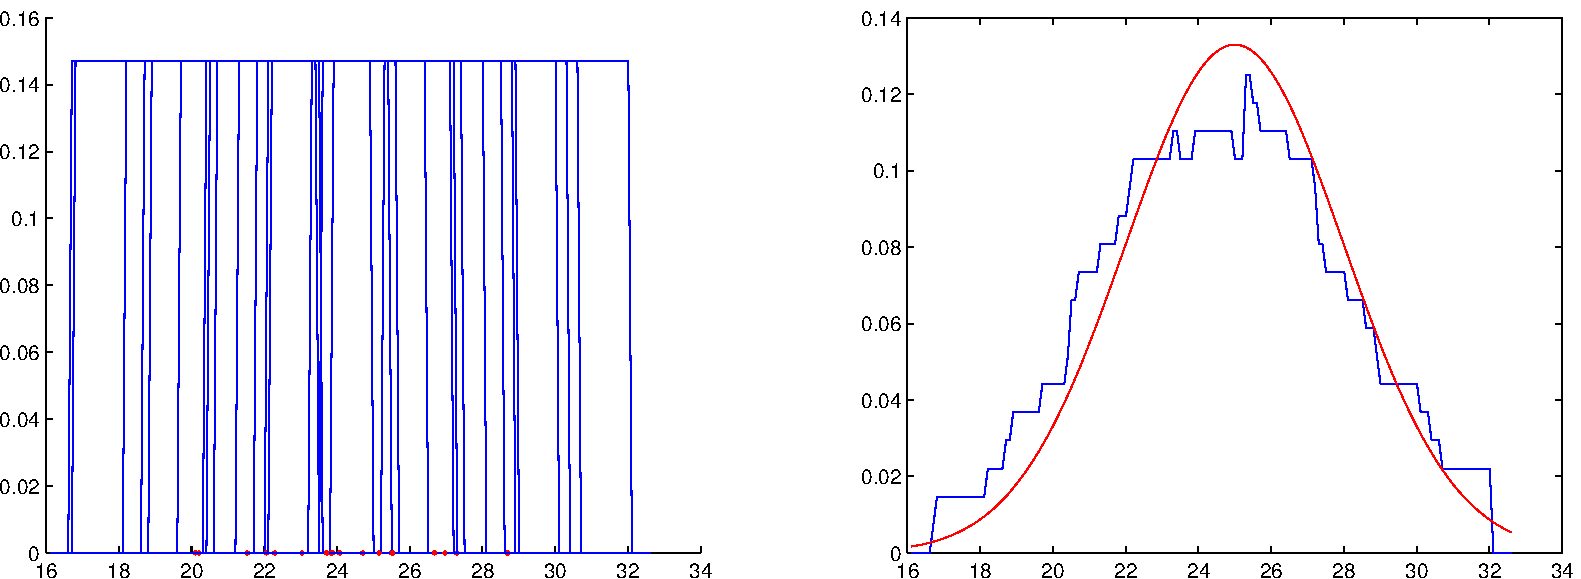
\includegraphics[width=0.8\textwidth]{img/parzen_2}
\end{figure}

En Matlab:

\begin{matlabcode}
for i=1:length(x)
  h = h + unifpdf(eje_x, datos(x) - ancho / 2, datos(x) + ancho / 2);
end
\end{matlabcode}

\subsubsection{Cálculo bidimensional}

De igual manera que en una dimensión, es posible utilizar el método de las
ventanas de Parzen para estimar la función de densidad de probabilidad de una
distribución bidimensional. La mecánica es básicamente igual que en una
dimensión.

\begin{matlabcode}
function r = Parzen2D(x,y,sigma,xi,yi)
%Parzen2D Estima la func de densidad en los puntos (xi,yi) mediante ventanas de
% Parzen centradas en los datos x,y

% Por cada clase
for i=1:max(y)
    
    % Aislamos los patrones de esa clase
    xAux = x(:, y == i);
    
    % Contenedor para las gausianas
    hAux = zeros(1,length(xi(:)));
    
    % Por cada patron
    for j=1:length(xAux),
        % Agregamos una gausiana centrada en ese patron
        hAux = hAux + mvnpdf([xi(:) yi(:)], xAux(:,j)', [sigma 0;0 sigma]')';
    end
    
    % Normalizamos y metemos en el contenedor de gausianas
    h(i,:) = hAux' / size(xAux,2);    
end

r = h;
end  
\end{matlabcode}

Una posible forma para utilizarlo en un problema de clasificación podría ser la
siguiente:

\begin{matlabcode}
[x,y] = shuffle(x,y);
  
xtrn = x(:, 1:100);
ytrn = y(:, 1:100);

xtst = x(:, 101:end);
ytst = y(:, 101:end);
 
h = Parzen2D(xtrn, ytrn, 0.7, xtst(1,:), xtst(2,:));
  
for i=1:3
  % Multiplicamos por las probabilidades a priori
  h(i,:) = h(i,:) * (length(xtrn(ytrn == i)) / length(xtrn)); 
end

% Nos quedamos con la clase con mayor densidad en cada punto
[~, pos] = max(h);
num_errores = sum(pos ~= ytst);
\end{matlabcode}

\end{document}